\chapter{Desenvolvimento}\label{cap2}
 Nesse capítulo será apresentado o projeto do EmerVant em suas áreas e escopo que irá atender. Também nesse capítulo  são apresentados o planejamento do projeto com base nesse escopo. Assim esse capítulo possui as seguintes seções:

\textit{Escopo} : Seção que apresenta o escopo do projeto, como os requisitos a serem atendidos.

\textit{Estrutura analítica do Projeto (EAP)}: Seção que descreve uma  EAP de modo a planejar as entregas ao longo do ciclo de vida do projeto.

\textit{Cronograma}: Seção que aborda o planejamento em atividades e datas assim como o gráfico de Gantt.

\textit{Solução inicial}: Seção na qual há uma proposta de solução inicial embasada em pesquisas gerais relacionadas ao produto.

\textit{Solução Técnica}: Seção que apresenta as soluções mais robustas e técnicas dadas ao projeto com base nas áreas definidas na EAP.

A solução técnica é apresentada nas seguintes subseções baseadas nas áreas definidas na EAP

\textit{Estrutura do VANT}: Essa subseção descreve o VANT em suas questões estruturais, tais como: dimensão, materiais, carga. Também aborda a escolha da aeronave e a especificação do tipo escolhido.

\textit{Sistema de Controle do VANT}: Nessa subseção estão descritas as formas de controle do VANT através da central de atendimento e como é dada essa comunicação entre a central e o VANT.

\textit{Comunicação do VANT}: Nessa subseção estão descritas as formas de comunicação entre o VANT e controlador, entre o VANT e o usuário-cidadão e entre o VANT e o usuário-central de atendimento.

\textit{Equipamentos de socorro}: Nessa subseção são apresentadas descrições e dimensões dos dois equipamentos a serem levados no VANT, o desfibrilador e o reanimador manual.

\textit{Sistema de Fornecimento de Energia}: Nessa subseção é abordado acerca de baterias em geral, como fonte energética selecionada, e da bateria escolhida para o projeto.


 \section{Escopo}
  \label{escopo}
Para definição do escopo do projeto foram analisados os seguintes aspectos: Local de atuação, localização da apoio, situações de socorro pré-hospitalar, viabilidade dos itens a serem levados pelo VANT, elementos estruturais e planejamento de atuação e estratégia de voo do VANT e o método de comunicação com o usuário.
\begin{description}
  \item[Local de Atuação] \hfill 
  	\begin{itemize}
  		\item Na Esplanada seja por natureza ou circunstância e será acionado apenas quando houver necessidade. Essa escolha foi realizada devido à grande circulação de pessoas e aos eventos esportivos e de entretenimento que ocorrem nesse local.

  	\end{itemize}
  \item[Tipo de emergência] \hfill 
  	\begin{itemize}
  		\item Paradas/Ataques Cardíacos;
		\item Paradas Respiratórias;
  	\end{itemize}
  \item[Equipamentos Utilizados para salvamento] \hfill \\
  	Para definir os itens a serem levados foi realizada uma análise de viabilidade levando em consideração a utilização dos equipamentos por pessoas sem conhecimento em salvamento e a possibilidade de carga útil do VANT.
  	\begin{itemize}
%   		\item Kit primeiro socorros;
		\item Desfibrilador Automático;
		\item Reanimador ventilatório manual;
  	\end{itemize}
  \item[Distância de Operação] \hfill 
  	\begin{itemize}
	  \item O VANT operará em um raio máximo de 10 km, para atender toda a esplanada.
	  \subitem Ele partirá de uma base fixa localizada no próprio batalhão do corpo de bombeiros da esplanada.

	\item A velocidade máxima do VANT é 60 km/h.
	  
  	\end{itemize}
  \item[Sinais vitais que serão monitorados] \hfill 
  	\begin{itemize}
	
	  \item Serão monitorados os batimentos cardíacos, os níveis de oxigenação no sangue. Esses sinais são essenciais para verificar o estado do paciente, com eles é possível ter uma conclusão do que aconteceu com a vítima. 
	    \subitem Eletrocardiograma (ECG)
	    \subitem Oxímetro.
  	\end{itemize}
  \item[Projeto mecânico estrutural] \hfill 
  
      Para atender todas as especificações e requisitos do projeto é necessário desenvolver o projeto estrutural completo do veículo, para esse projeto foi levado em consideração os possíveis materiais e o tipo de estrutura que melhor atende as necessidades do projeto.
  	O VANT será:
  	\begin{itemize}
  		\item de asa rotativa,pois necessita-se de um voo mais estável e uma maior versatilidade de pousos e decolagens;
		  \subitem Octacóptero.
		\item elétrico, devido a maior eficiência e maiores rendimentos em termos energéticos.
  	\end{itemize}
  \item[Materiais] \hfill 
  
  Os materiais da estrutura foram escolhidos por serem componentes versáteis e com propriedades importantes para a construção da estrutura mecânica do VANT. As propriedades que levaram a escolher esses materiais foram a grande resistência mecânica e baixo peso:
  	\begin{itemize}
  		\item Polímeros compostos;
		\item Fibra de carbono.
  	\end{itemize}
  \item[Controle] \hfill 
  	\begin{itemize}
  		\item O Controle do VANT será através de uma placa controladora, com ela é possível a implementação do automático e o comando partindo da central de comunicação. 
  		Será estabelecido uma forma de comunicação entre o VANT e a central de controle.
  		A central passará as coordenadas e poderá visualizar todas as partes do atendimento, isso é: O deslocamento do VANT até o paciente e os procedimentos realizados. 
  	\end{itemize}
  \item[Comunicação entre equipe de paramédicos e usuário] \hfill 
  	\begin{itemize}
  		\item Câmera e sistema de áudio. Sendo que, o vídeo será apenas para o paramédico da central e a comunicação via áudio para ambos;
  		\item O usuário apenas escutará as instruções, comunicando-se apenas através do áudio.
  	\end{itemize}
  	
  \item[Massa máxima total do sistema]\hfill
	  	\begin{itemize}
  		\item 12 Kg.

  	\end{itemize}
\end{description}

\section{Estrutura Analítica de Projeto - EAP}
  
No desenvolvimento de qualquer projeto, é essencial ter uma visão geral sobre as atividades que serão realizadas no decorrer da processo de criação.  Para isso existem formas de sistematização e organização dessas informações.

Uma dessas formas de organizar a informação é a EAP - Estrutra Analítica do Projeto - que é a estruturação das entregas a serem completadas em forma de árvore de maneira hierárquica, onde são distribuídas da mais gerais para as mais especificas.

A EAP foi a forma escolhida pela equipe de desenvolvimento do projeto EmerVant para estruturação das entregas, por proporcionar de uma maneira simples e objetiva todos os pontos abordados e discutidos para a realização do projeto em seu devidos graus de importância. 

Para a criação da EAP do EmerVant, foi observado que dentro do projeto há varias áreas de atuação. Assim os níveis mais gerais foram definidos por essas áreas de atuação que são:
\begin{itemize}
\item Gerência de Projetos;
\item Iniciação;
\item Estrutura do VANT;
\item Comunicação;
\item Controle;
\item Fonte Energética;
\item Encerramento.
\end{itemize}
As entregas especificas de cada tópico foram baseadas nas definições de escopo e requisitos. A Figura \ref{fig:eap} é a representação gráfica da EAP criada para o projeto EmerVant.
% \begin{figure}[h!]
%  \flushleft
%     % 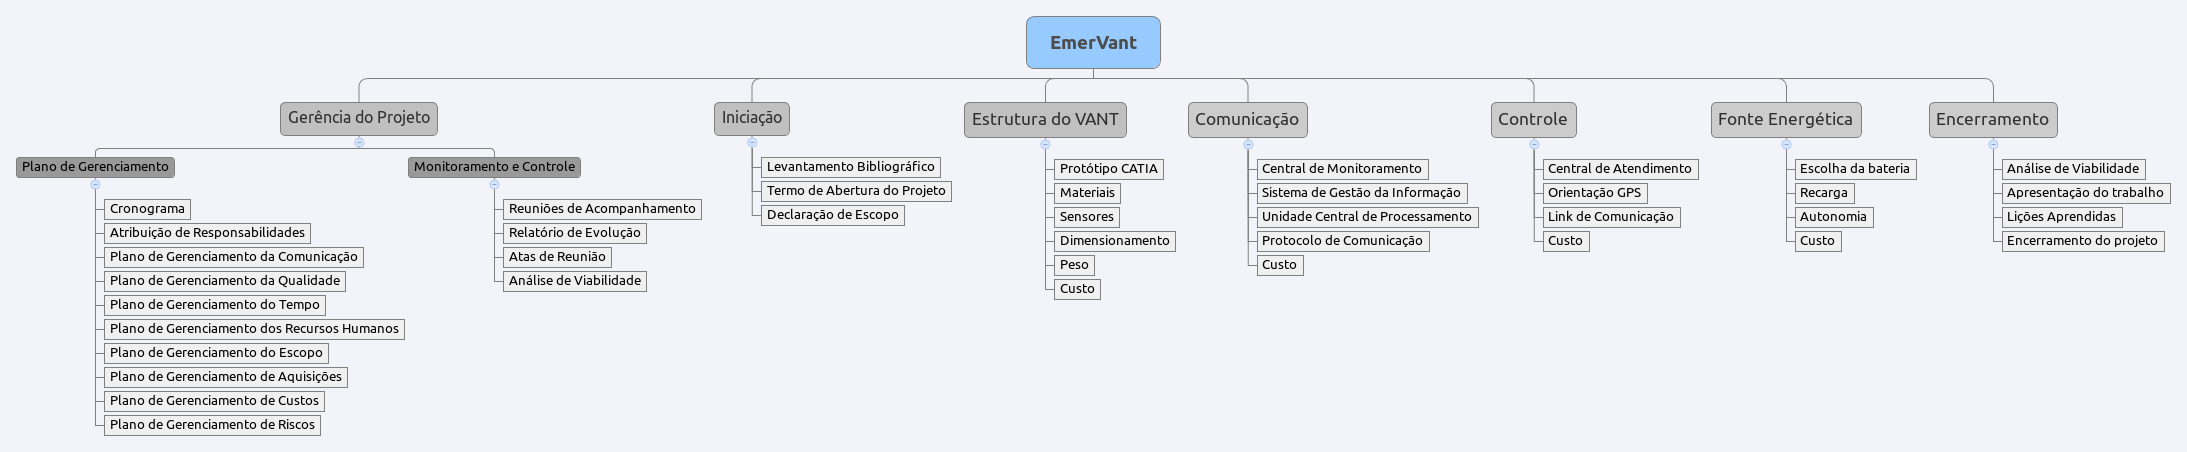
\includegraphics[keepaspectratio=true,scale=0.4]{figuras/eap.png}
%     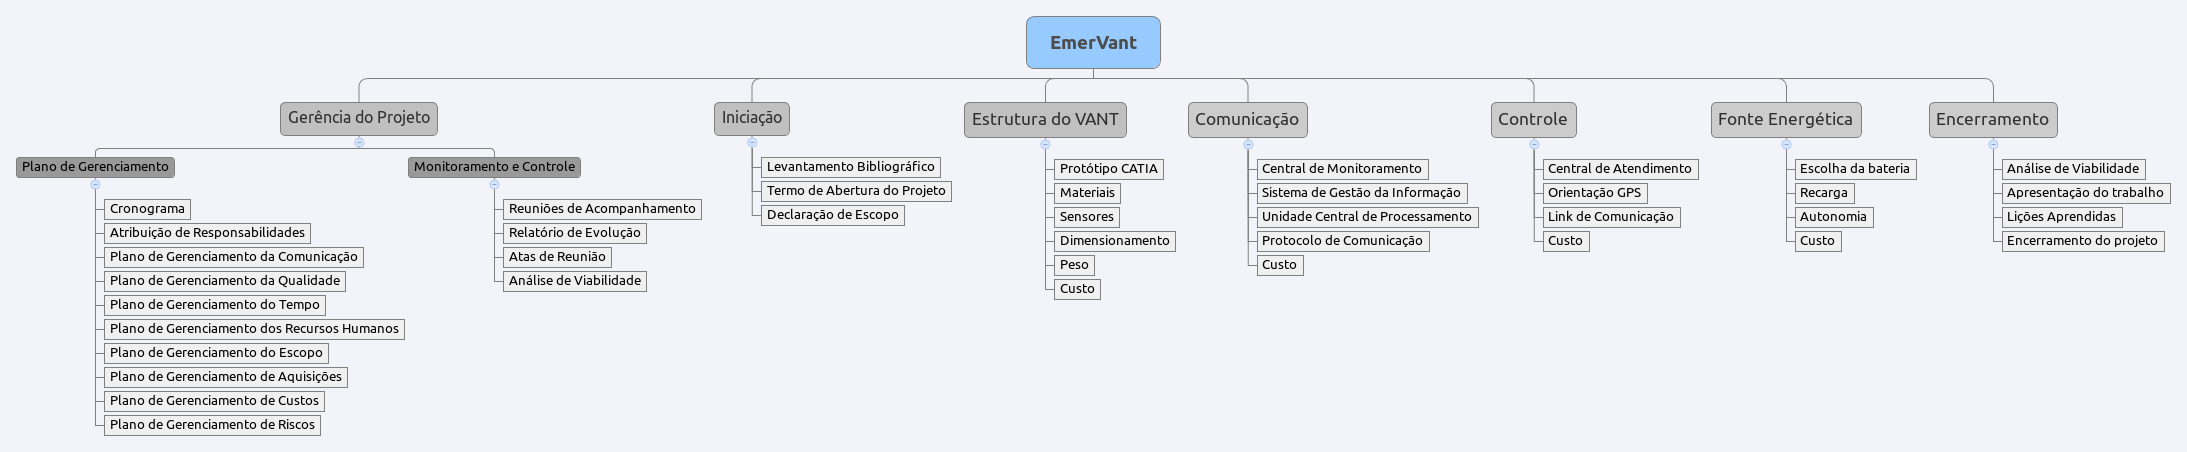
\includegraphics[height=6cm,width=18cm]{figuras/eap.eps}
%   \caption{Estrutura Analítica do Projeto EmerVant}
%   \label{fig:eap}
% \end{figure}
\vfill
\pagebreak

 
\pagebreak
\section{Cronograma}
  O cronograma preliminar das atividades foi baseado de acordo com os prazos para entrega dos relatórios parciais em cada ponto de controle. 
Também foi levado em consideração a responsabilidade por cada atividade.
Com o cronograma estabelecido, pode ser elaborado o gráfico de Gantt Figura \ref{fig:gantt}, no qual podemos observar o
tempo de execução de cada atividade desenvolvida nas várias etapas do projeto. 
% 
% \vfill
 \begin{figure}[!ht]
	\centering
		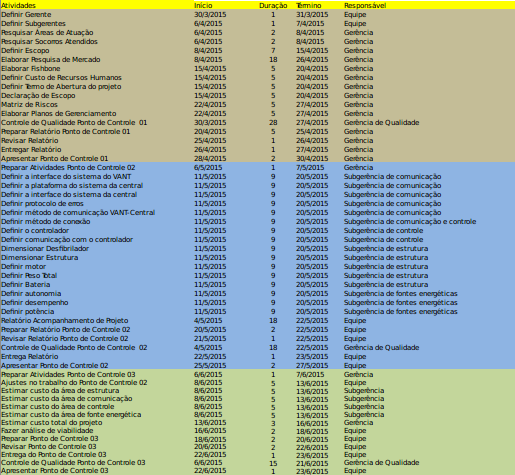
\includegraphics[keepaspectratio=true,scale=0.9]{figuras/cronograma.png}
	\caption{Cronograma de Atividades}
	\label{fig:cronograma}
\end{figure}

 \begin{figure}[H]
	\flushleft
		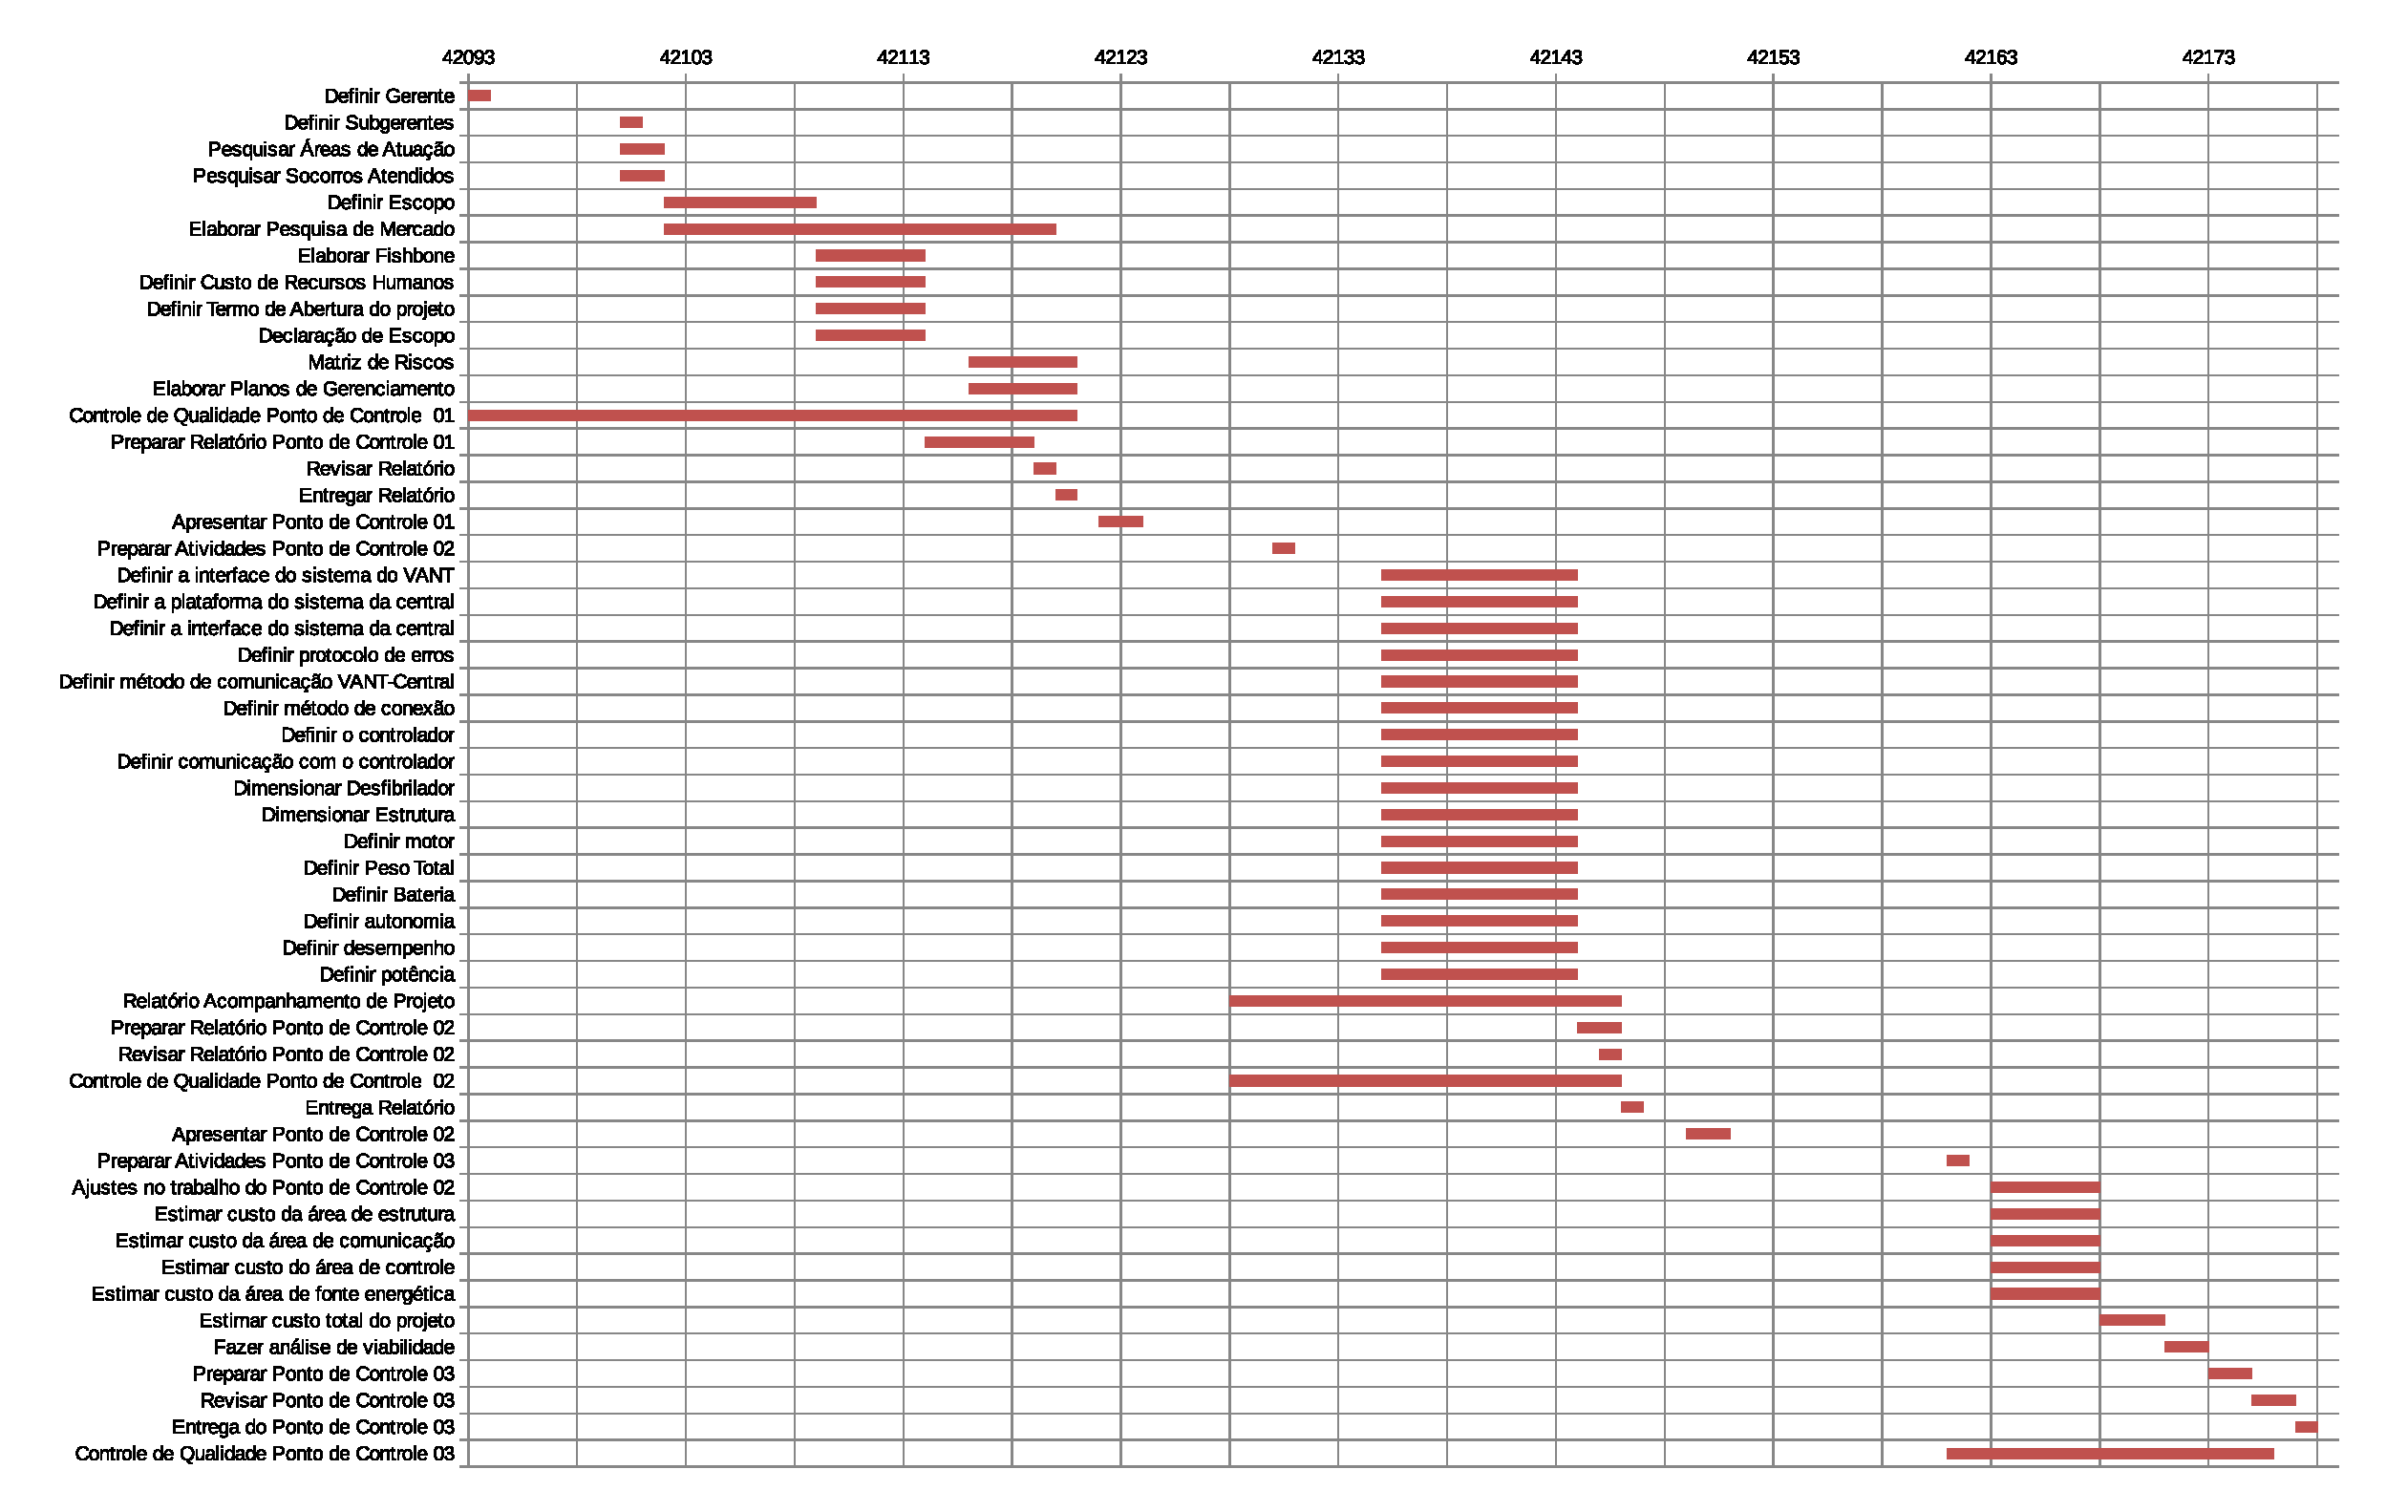
\includegraphics[height=13cm,width=18cm]{figuras/gantt.eps}
	\caption{Gráfico de Gantt}
	\label{fig:gantt}
\end{figure}


\section{Solução Inicial}
  O EmerVant consiste em um sistema de assistência emergencial através da utilização de um VANT.	

O grande potencial dos drones tem sido explorado em inúmeras implementações militares e civis. Entre os vários VANTs, estes de pequena escala são atraentes para o meio acadêmico, devido ao seu pequeno tamanho, as capacidades de voo único, excelente dirigibilidade e baixo custo. \cite{SDM}.

O VANT escolhido para a aplicação foi o multirotor de oito hélices, conhecido como octocóptero. Usando um essa configuração a força de sustentação é melhor dividida entre os múltiplos motores possibilitando carregar uma maior carga útil e tendo uma maior estabilidade.

O \textit{Global Position System} (GPS) é o sensor de maior importância deste projeto, pois as informações fornecidas serialmente por esse componente auxiliam não só na estabilização da aeronave mas no controle e na locomoção do VANT até o local desejado.

Em uma situação normal o desempenho do piloto automático excede a que é controlada por humanos, e mesmo em situações mais desafiadoras sua performance é equivalente.

O projeto mecânico estrutural será constituído de polímeros compostos e fibra de carbono. O VANT será de asa rotativa e utilizará alguns sensores que serão processados por sistemas embarcados dedicados ao voo. 

O controle será feito através de um sistema automático com o uso de GPS, utilizado para deslocamento e localização. Através desse sensor o piloto automático tem acesso às informações em tempo real, utilizando-as ele consegue guiar-se, dessa maneira ele sabe exatamente seu lugar no espaço e sua localização à obstáculos. Para gerar essas informações são necessários: giroscópios, acelerômetro, sensores magnéticos e eletromagnéticos, sensores visuais, sensores ultrassom, infravermelhos, micro-ondas e gamas de rádio. \cite{UDE}

Seu local de atuação será na Esplanada dos Ministérios. Quando acionado a central, que fica em um ponto estratégico da Esplanada, irá receberá a informação referente a necessidade e irá passar de forma serial para o drone as coordenadas referentes  ao local e situação da(s) vítima(s).

O monitoramento do VANT ocorrerá através de um sistema de controle automático por rádio frequência que será monitorado e comandado pela central de monitoramento. Ele terá uma câmera e um sistema de áudio.

O VANT, através da câmera e do sistema de áudio estabelecerá a comunicação entre o usuário,a ambulância e a central de monitoramento. O vídeo será apresentado apenas para o paramédico da central e o áudio para a central e a ambulância. O contato do usuário será apenas com o áudio.

O paramédico dará orientações para quem está com a vítima através do sistema de comunicação do EmerVant. Com a câmera os paramédicos da central de comando poderá visualizar a situação, dar instruções para utilizar o desfibrilador ou reanimador ventilatório manual. 


\section{Solução Técnica}
  Nessa seção serão apresentadas as soluções técnicas de cada área definida na EAP: estrutura do VANT,
  fonte energética do VANT, Controle e Comunicação.

\subsection{Estrutura do VANT}
  Essa seção apresenta a estrutura geral do VANT como aeronave escolhida, seus materiais e seu protótipo.
\subsubsection{Escolha da aeronave}

Para escolha da aeronave, que atende à todas as necessidades impostas pelo projeto, deve-se considerar quais características a aeronave possui.
A escolha levou em consideração a melhor aeronavegável e que pudesse suportar a maior carga possível.

O VANT precisa atender o transporte de equipamento hospitalar, as possíveis aeronaves para essa função são: VANT asa fixa e VANT asa 
rotativa (multirotores).

Os VANT’s de asa fixa, no caso, os aviões não tripulados, apesar de serem rápidos e possuírem um longo alcance de voo, para transporte de carga,
exige um tamanho grande de asa, A envergadura do VANT muda com relação ao peso, e como a carga de transporte é considerada elevada, o 
comprimento da asa teria que ser muito grande, como o próprio avião. A aterrisagem é outro fator que dificulta, pois os aeromodelos 
exige um espaço aberto com uma pista de pouso para conseguirem descer. As dimensões da pista é uma grande dificuldade, pois a pista
precisa ser maior que o modelismo e não é em qualquer lugar que ele pode realizar esse procedimento, devido o grande risco,
tornando-se perigoso. Não é aconselhado pousos próximo de pessoas e em curtos espaços.

Os multirotores vêm aumentando no mercado nos últimos anos. Os multirotores são estruturas com vários motores (dois ou mais rotores) e 
esses motores são fixos em uma estrutura, e os motores não precisão de ajustes como nos helicópteros. O \textit{Roll} e o \textit{Pitch} é feito 
apenas com a rotação do motor. Além disso, não há rotor de cauda, utilizada para fornecer controle de guinada e contrariar o torque posto 
para fora por dirigir o principal rotor em um helicóptero. Por serem simétricos, o controle de um multirotor é mais fácil e mais estável. O
que permite uma decolagem e uma aterrissagem mais prática e com menos espaço.

Os multirotores voam através da utilização de dois princípios básicos: elevação (\textit{lift}) e torque. Multirotores são verdadeiramente
um grande exercício de física newtoniana: toda ação tem uma reação de mesma intensidade e sentido oposto. O multirotor usa  hélices 
diferentes e a contra-rotação para  manter o corpo  estável, pois dessa forma mantem-se a conservação do momento angular \cite{audronis}. 
Nos helicópteros tem-se o rotor de calda para evitar que o corpo girar e perca a estabilidade, o rotor de cauda é implementado de forma que 
mantenha a conservação de momento no helicóptero. 

Na figura \ref{fig:rotacao} é possível ver um multirotor, a representação mostra como que as hélices devem girar para que seja possível 
um voo estável. Esse princípio é aplicado a todos os multirodores e não apenas no quadrirotor. Sempre as hélices opostas (as que ficam 
uma em frente da outra) devem girar em mesma direção caso deseja-se entrar para frente.


\begin{figure}[H]
    \centering
      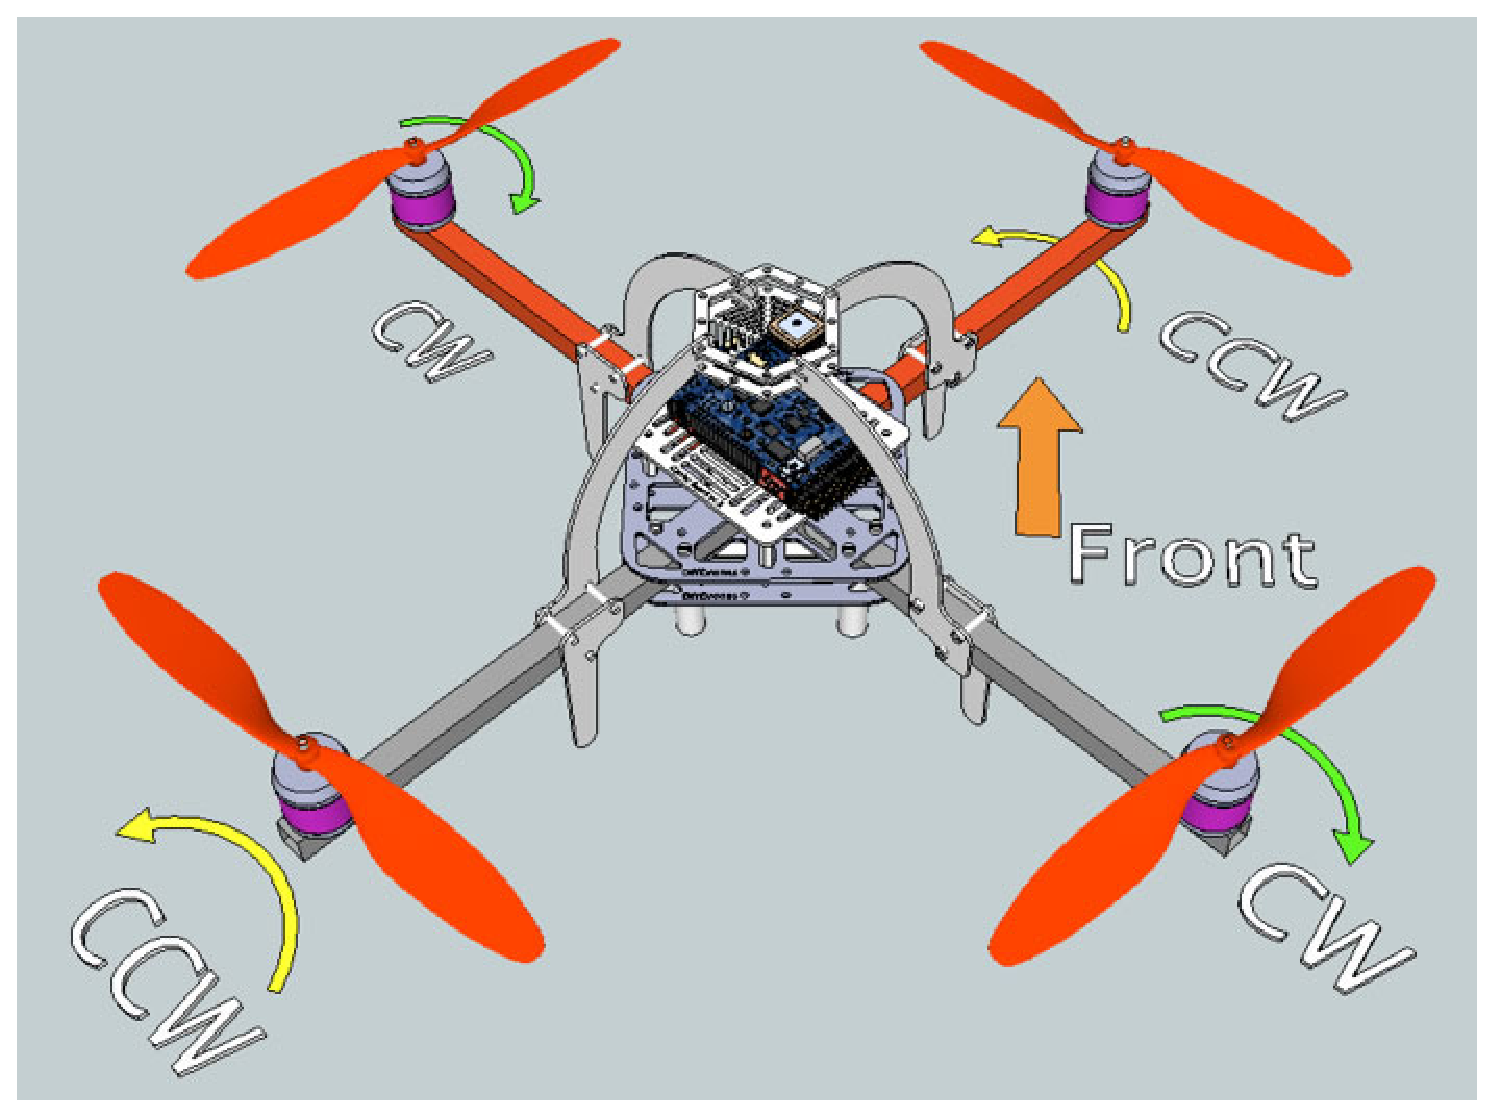
\includegraphics[keepaspectratio=true,scale=0.5]{figuras/rotacao.eps}
    \caption[Diagrama  de rotação das hélices de um quadricoptero estável]{Diagrama  de rotação das hélices de um quadricoptero estável. Fonte \cite{audronis}}
    \label{fig:rotacao}
\end{figure}

O multirotor possui a mobilidade de ir para frente, para trás e de lado para o outro mudando apenas o sentido temporariamente das hélices
como representado na imagem \ref{fig:gira}. Ao realizar essas manobrar ele pode inclinar o multirotor, alterando a direção do empuxo fornecido 
pelos rotores dessa forma realizando a curva mostrado na imagem \ref{fig:guinada}.

\begin{figure}[H]
    \centering
      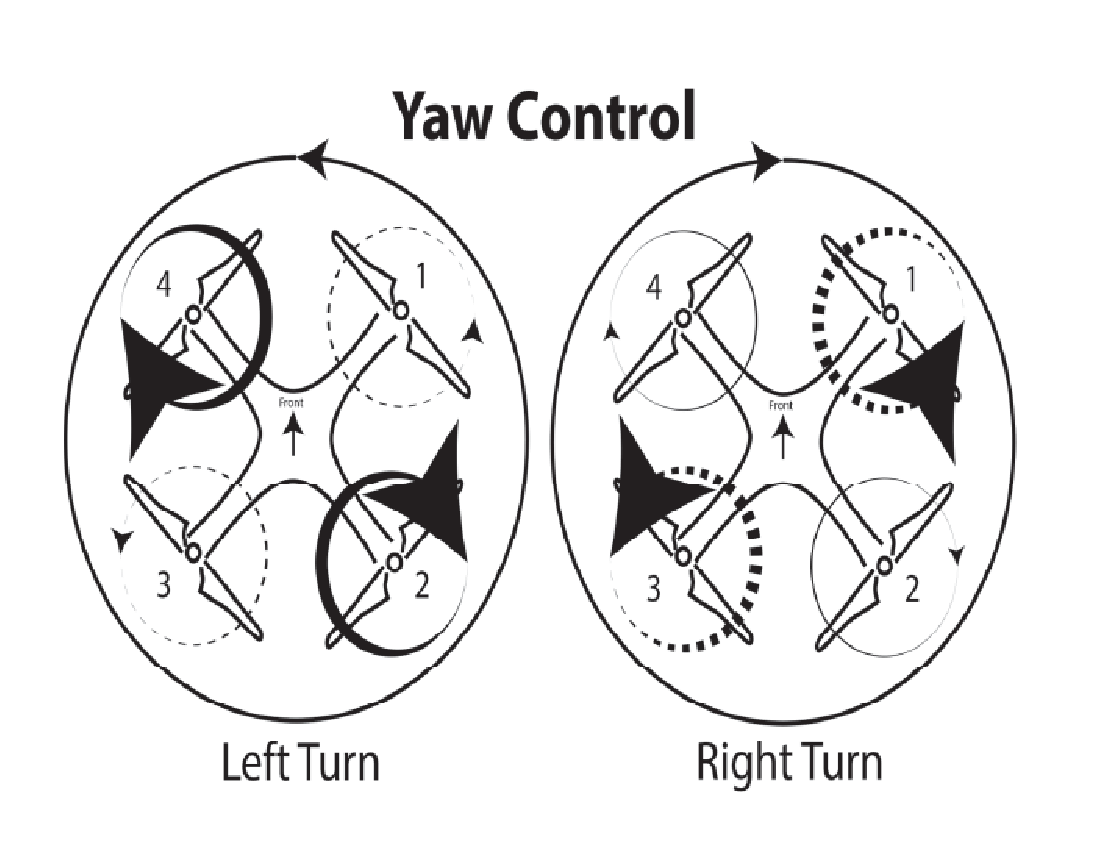
\includegraphics[keepaspectratio=true,scale=0.5]{figuras/gira.eps}
    \caption{Diagrama de gira para esquerda e para direita. Fonte \cite{audronis}}
    \label{fig:gira}
\end{figure}

\begin{figure}[H]
    \centering
      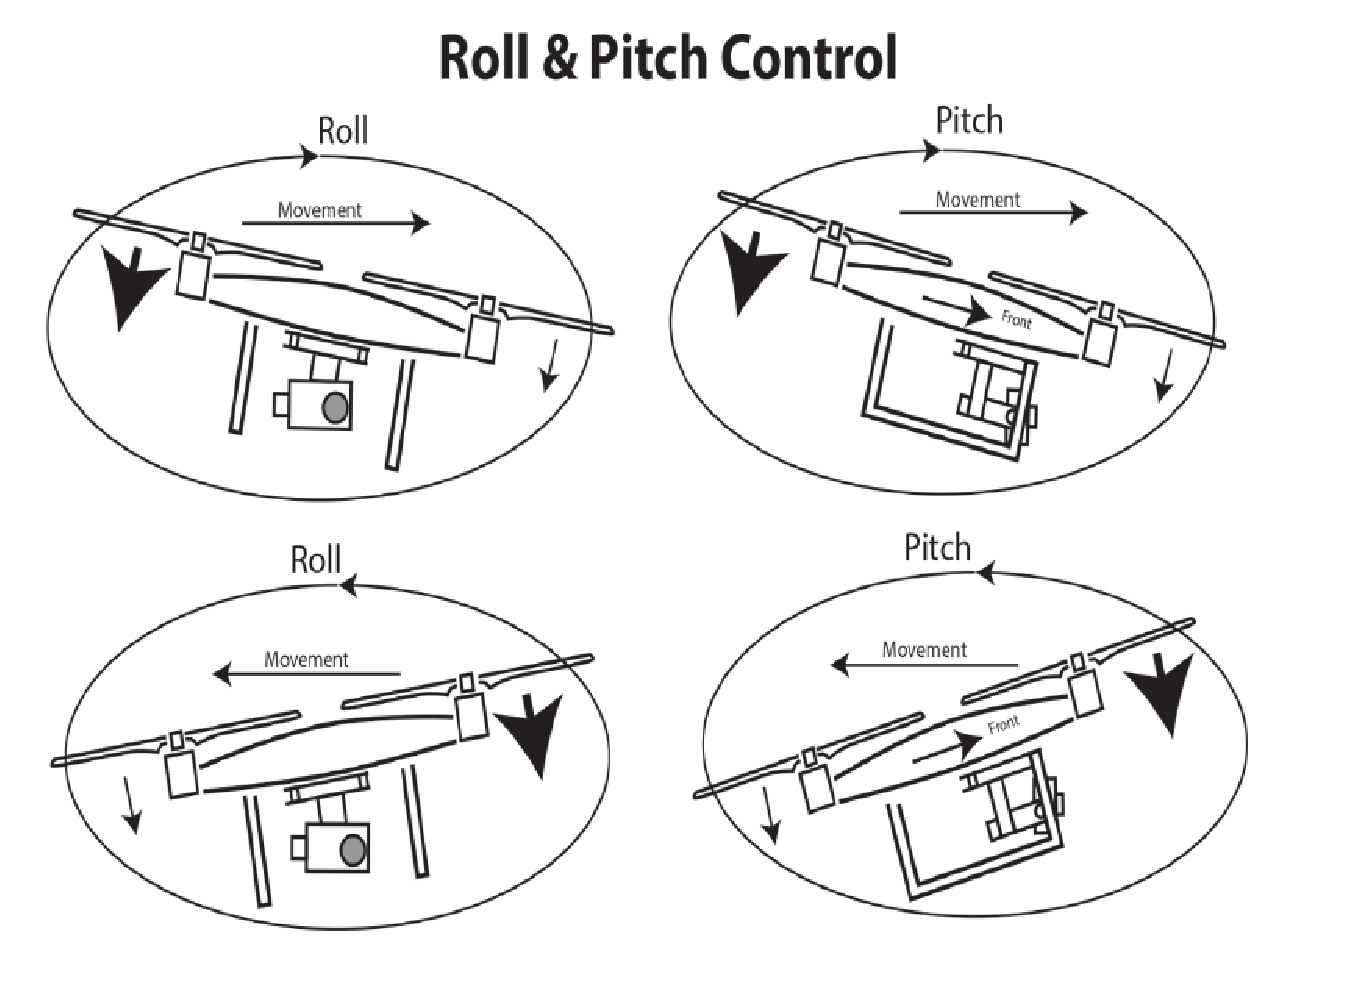
\includegraphics[keepaspectratio=true,scale=0.5]{figuras/guinada.eps}
    \caption[Diagrama de guinada e rolagem de um quadricóptero.]{Diagrama de guinada e rolagem de um quadricóptero. Fonte \cite{audronis}}
    \label{fig:guinada}
\end{figure}
A desvantagem de utilizar  os multirotores  é a  falta  de aerodinâmica,  dessa for o tempo de voo é reduzido significativamente e a baixa  
eficiência dos motores.  Contudo, para transporte de equipamento hospitalar, mas para o projeto será ideal, pois sua estabilidade, 
facilidade de controle, o tamanho reduzido e grande mobilidade compensa a falta de eficiência. A aplicação não precisa de percorrer 
distâncias muito grande, com isso ele se encaixa perfeitamente nas especificações.
\subsubsection{Especificação do VANT escolhido}

O multirotor escolhido para esse projeto é o de oito hélices, ou octocóptero. Em- bora oito rotores ofereçam mais estabilidade, também diminuem 
o tempo de voo, porque aumenta a quantidade de corrente exigida para alimentar todos os motores.  O projeto exige uma maior capacidade de carga, pois os equipamentos utilizados são considerados de alta densidade. Para que as especificações fossem atendidas, decidiu-se utilizar essa especificação por sua estabilidade e maior capacidade de gerar empuxo.

O motor escolhido é o motor Tarot 4114 \textit{High Power Brushless} (sem escova), que é um motor de altas rotações, representado na figura 
\ref{fig:tarot2}.

\begin{figure}[H]
    \centering
      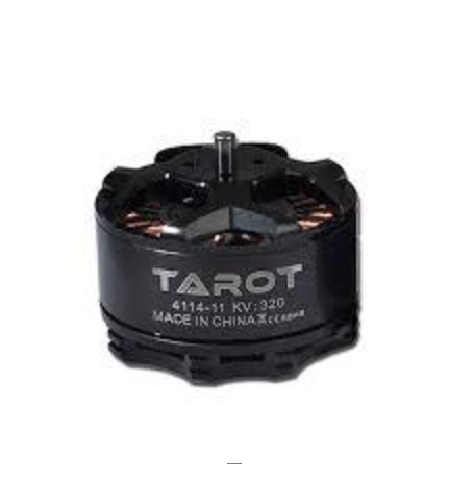
\includegraphics[keepaspectratio=true,scale=0.5]{figuras/tarot2.eps}
    \caption{Motor Tarot 4114 \textit{High Power Brushless}. \cite{tarot}}
    \label{fig:tarot2}
\end{figure}
\vfill
Este motor é comumente utilizado em  multirotores, um exemplo o modelo US 1000 de filmagens. Ele possui capacidade de gerar um empuxo de até
2.5 kg e uma outra característica desse tipo de motor é a magnetização do rotor ser por imãs permanentes. Motores de corrente contínua 
possuem vários benefícios em relação aos motores com escova, dentre algumas estão: melhor característica velocidade x torque, maiores
eficiência, vida útil, taxa de velocidade e é mais silencioso \cite{nascimento}.

\begin{figure}[H]
    \centering
      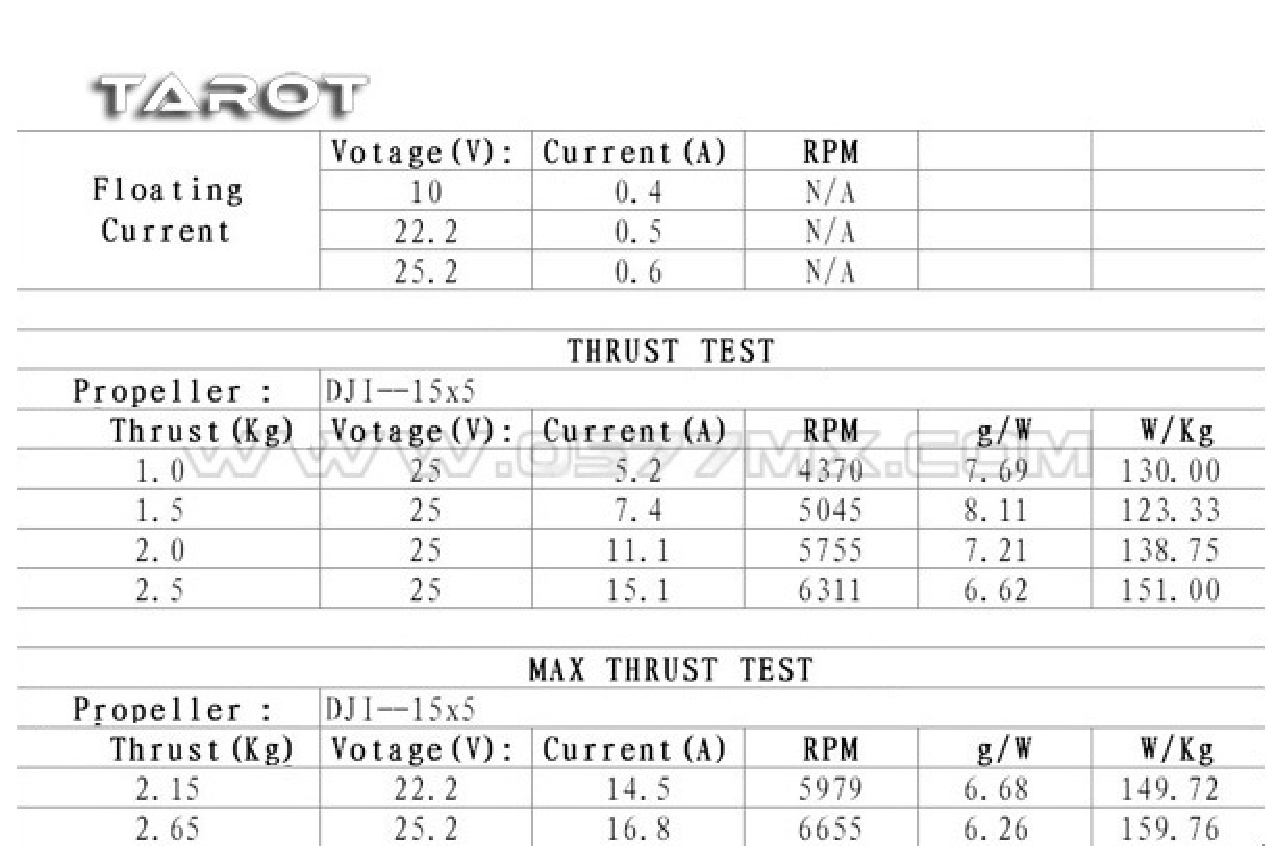
\includegraphics[keepaspectratio=true,scale=0.5]{figuras/tarot.eps}
    \caption{Quadro de relação de um motor 4114.\cite{tarot}}
    \label{fig:tarot}
\end{figure}

A hélice é um conjunto de pás com o mesmo centro, que ao serem rotacionadas criam um deslocamento do ar em direção ao solo e pelo efeito da 
terceira lei de Newton o conjunto é impulsionado para o sentido oposto, dessa forma cria-se a sustentação necessária para o vôo.  
Quanto maior o passo da hélice, maior a velocidade alcançada  pela aeronave e mais lenta é a resposta à manobras \cite{VIOLATO}. 
Para nossa proposta, utilizou-se uma hélice de tamanho médio, pois a aplicação necessita de velocidade e também de uma mobilidade boa.
A hélice escolhida é a 15x5 5.E \textit{Carbon  Fiber  Propellers  L/H  and  R/H  Rotation  Suits DJI}.

\begin{figure}[H]
    \centering
      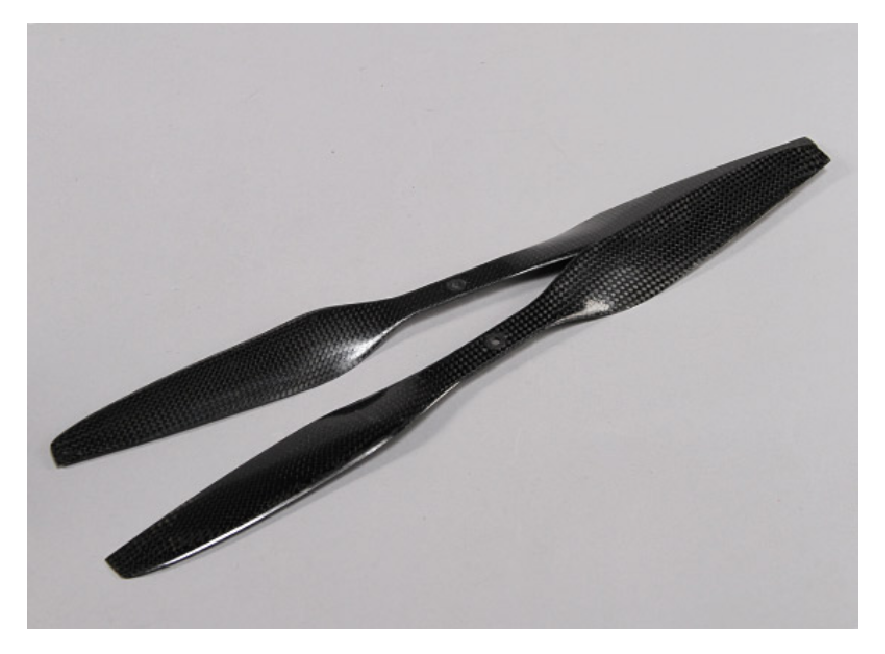
\includegraphics[keepaspectratio=true,scale=0.5]{figuras/diagramaEstru.eps}
    \caption[\textit{Carbon Fiber Propellers L/H and R/H Rotation Suits DJI.}]{\textit{Carbon Fiber Propellers L/H and R/H Rotation Suits DJI.} \cite{pinto}}
    \label{fig:elice}
\end{figure}

O ESC (\textit{Eletronic speed control}) é quem torna possível o voo, é o controle eletrônico da velocidade, ele é o responsável por 
alimentar o motor e mandar a potência que é necessária, ele impede sobrecarga nos motores, funcionando também como um módulo de proteção. 
Os ESCS são específicos para cada motor, eles devem ser dimensionados corretamente, pois um dimensionamento indevido pode ocasionar em uma 
sobrecarga nos motores e queimá-los.  Cada motor tem o seu ESC individual, dessa forma é possível controlar individualmente cada motor. Os 
ESCs são ligados no circuito do VANT como mostra a figura \ref{fig:diagramaEstru}.
 

\begin{figure}[H]
    \centering
      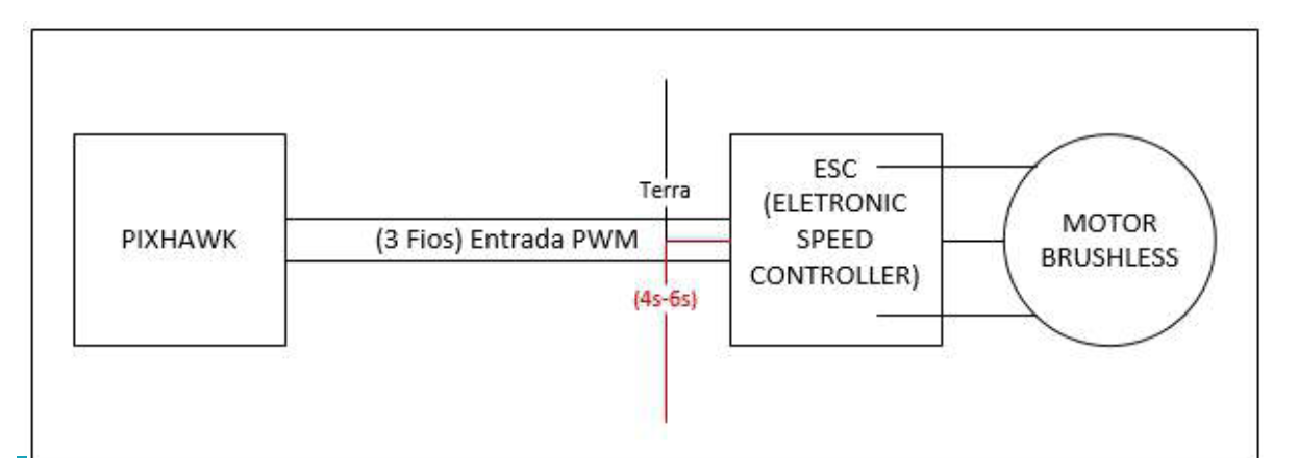
\includegraphics[keepaspectratio=true,scale=0.5]{figuras/elice.eps}
     \caption{Esquemático  de conexão e funcionamento  do ESC\cite{dji}}
    \label{fig:diagramaEstru}
\end{figure}

\subsubsection{Escolha dos materiais}

A escolha de determinados materiais nos projeto da engenharia é determinante para um bom projeto, para a escolha leva-se em  consideração 
os ambientes em que serão operados, dessa forma é possível entender o comportamento dos materiais diante a aplicação, dessa forma podendo 
garantir uma maior solidez e confiabilidade no projeto.

Os componentes que farão parte do drone serão os motores de alto desempenho, as hélices, componentes elétricos e a estrutura do corpo. 
Esta delimitação de materiais que satisfazem as necessidades do drone foi feita levando  em conta o tipo dos esforços que estarão  presentes,  
por exemplo, na decolagem, aterrissagem  e durante o tempo  de voo. Para as hélices e para  o motor foi escolhida  a fibra de carbono  e
para  o restante dos materiais da estrutura a opção foi da fibra de vidro.

A justificativa para a escolha destes materiais foi baseada de acordo com o módulo de elasticidade, a ductilidade, o limite de
resistência à tração e a tenacidade. 

Para que seja possível a visualização da comparação feita, as características citadas acima serão brevemente explicadas.


\begin{figure}[H]
    \centering
      \includegraphics[keepaspectratio=true,scale=0.7]{figuras/grafico-tensao.eps}
    \caption{Gráfico Tensão-Deformação.Fonte: \cite{callister}}
    \label{fig:grafico-tensao}
\end{figure}

O módulo de elasticidade é a inclinação da região de comportamento elástico inicial da curva, ou seja, o coeficiente linear da reta antes de atingir a região de deslizamento de discordâncias.
\begin{equation}
E =\frac{\Delta y}{\Delta x}
\end{equation}
A ductilidade é a medida do grau de deformação plástico que foi suportada até a fratura(F). Pode ser expressa quantitativamente como a porcentagem do alongamento percentual.
\begin{equation}
AL\% =\frac{lf - lo}{lo} * 100
\end{equation}
\begin{center}
lf = comprimento final e lo = comprimento inicial
\end{center}

O limite de resistência à tração está caracterizado no gráfico como início da ruptura e indica o valor máximo de tensão que pode ser suportado por uma estrutura sob tração.
A tenacidade é definida como sendo a habilidade de um material absorver energia e se deformar plasticamente antes de fraturar.

\begin{figure}[h]
    \centering
      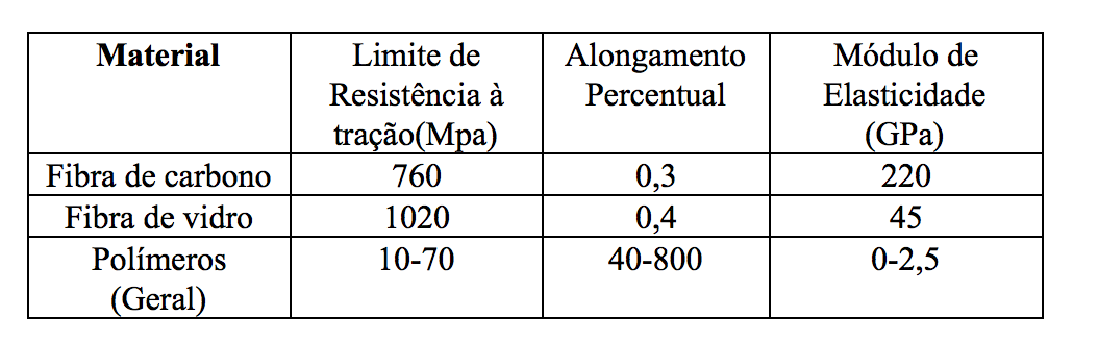
\includegraphics[keepaspectratio=true,scale=0.7]{figuras/graficoRelacao.eps}
    \caption{ Relação de materiais}
    \label{fig:graficoRelacao}
\end{figure}

Os materiais escolhidos, fibra de vidro e carbono, são determinados como materiais compósitos. As características destes incluem em pegar as melhores carcteristicas de variados materiais e junta-las para que se tenha um melhor desempenho no geral. 

Portanto, a escolha dos materiais do drone pode ser explicada de acordo com a tabela acima e com as explicações teóricas do que cada característica representa. 

Embora o alongamento percentual dos materiais poliméricos em geral seja muito maior do que os dos materiais ecolhidos para a aplicação do drone, esta característica é exibida no domínio plástico, ou seja, o material não se romperá mais perderá a qualidade devido a uma quantidade significativa de deformação.

Como conclusão do material a ser utilizado, é interessante partes da estrutura, como os braços, frame central, hélices e trem de pouso, utilizando fibra de carbono. Partes como a carcaça e componentes eletrônicos, poderão ser utilizados polímeros em geral. 

\subsubsection{Construção do VANT}

Considerando a parte mais importante do projeto, o desfibrilador será acoplado no VANT, na qual suas medidas são utilizadas como referência para modelagem do frame central.  A modelagem dos braços e hélices do drone,  não serão necessários, devido ao fato que eles serão utilizados do modelo similar ao de um VANT S1000

Para inicio da construção do VANT, consideramos as medidas de um DEA (Desfibrilador externo automático) vendido no mercado, chamado \textit{HeartSine samaritan PAD SAM 300P}  como o representado na figura \ref{fig:heart}:

\begin{figure}[H]
    \centering
      \includegraphics[keepaspectratio=true,scale=0.2]{figuras/heart.eps}
    \caption{ HeartSine samaritan PAD SAM 300P. Fonte: \cite{aedsingapore}}
    \label{fig:heart}
\end{figure}

O frame central projetado será baseado no frame central do S1000, porém adaptado ao desfibrilador e ao reanimador ventilatório, como é possível ver na figura 19: 

\begin{figure}[H]
    \centering
      \includegraphics[keepaspectratio=true,scale=0.5]{figuras/framecentral.eps}
    \caption{ Frame central S1000. Fonte: \cite{heliguy}}
    \label{fig:framecentral}
\end{figure}


Como as medidas, seguindo o manual, do frame central do S1000 é 337.5mm da ponta de um braço até outra, para o nosso projeto, será aumentado  200mm em relação ao centro, 100mm para um lado e 100mm par outro. Como mostra na figura \ref{fig:drawing}:

\begin{figure}[H]
    \centering
      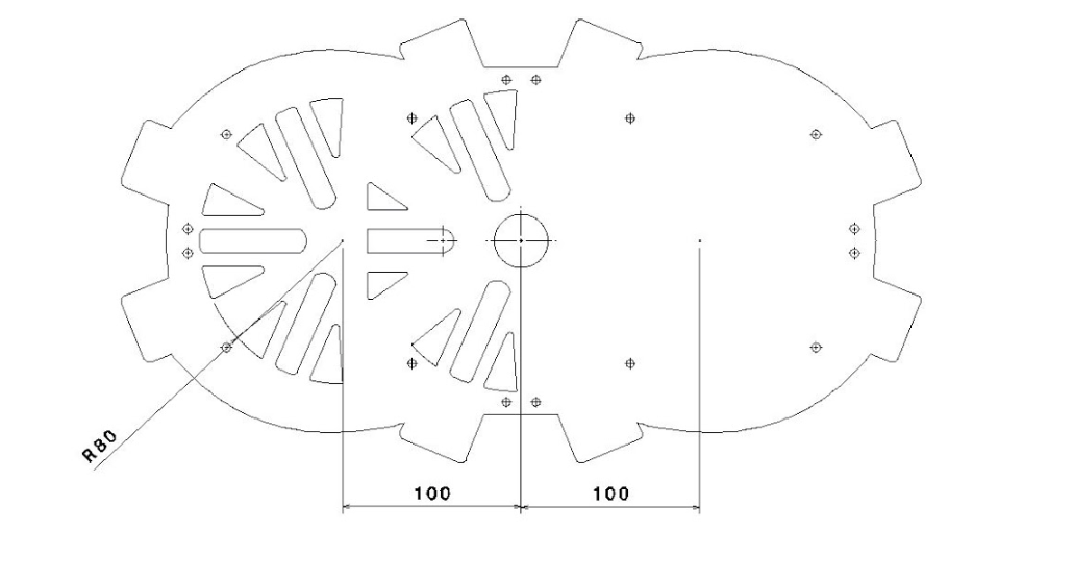
\includegraphics[keepaspectratio=true,scale=0.5]{figuras/drawing.eps}
    \caption{ Drawing Frame Central Superior}
    \label{fig:drawing}
\end{figure}

Como é possível ver na figura \label{fig:drawinfinfo}, as formas triangulares do lado esquerdo são “buracos” na qual tem como função deixar o frame mais leve, contudo, não perder sua utilidade em ser a base do VANT. O lado direito não possui esses espaços devido ser o local para alocar o desfibrilador. O lado esquerdo alocará a antena e até duas baterias , na qual serão presas por velcros, amarrados entre os “buracos” do frame. Também serão parafusadas os braços e a carcaça do VANT no mesmo.

\begin{figure}[H]
    \centering
      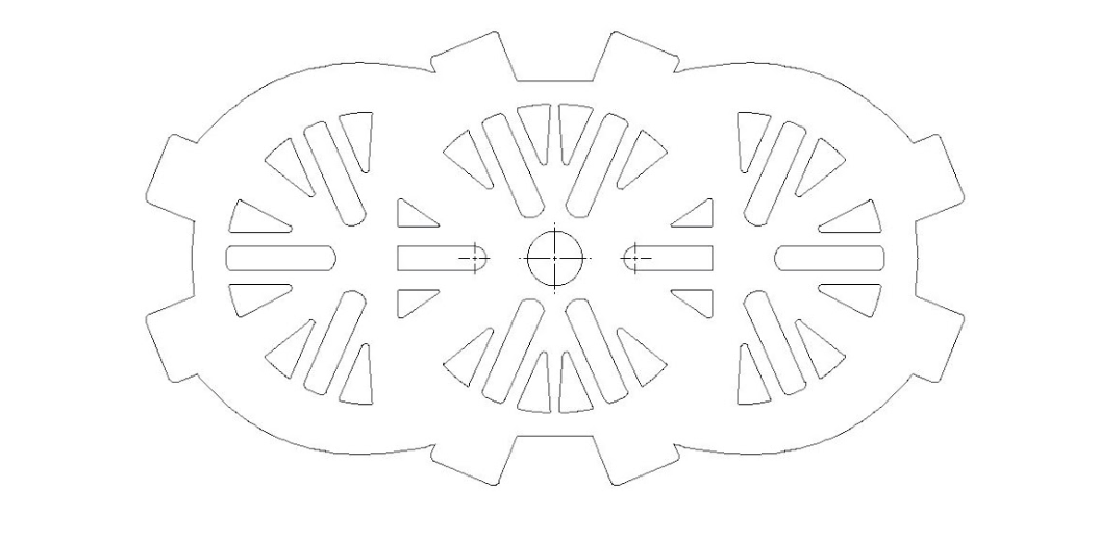
\includegraphics[keepaspectratio=true,scale=0.5]{figuras/drawinfinfo.eps}
    \caption{ Frame Central inferior.}
    \label{fig:drawinfinfo}
\end{figure}

Já o frame inferior, figura \ref{fig:drawinfinfo}, será parafusado ao trem de pouso e ao frame superior.  Ambos os frames serão unidos como mostra a figura \ref{fig:catia1}, tendo um espaço de 42mm. O espaço entre os dois frames é destinado para alocar a parte dos controladores de voo , ESC e o conjunto dos fios.

\begin{figure}[H]
    \centering
      \includegraphics[keepaspectratio=true,scale=0.5]{figuras/catia1.eps}
    \caption{Desenvolvimento do VANT no CATIA}
    \label{fig:catia1}
\end{figure}

Por meio da plataforma CATIA, foi possível idealizar o projeto EmerVANT, em escala real. Para visualizar de melhor forma, utilizou-se o KeyShot, na qual ele renderiza VANT, como mostrado na figura \ref{fig:keyshot1}:

\begin{figure}[H]
    \centering
      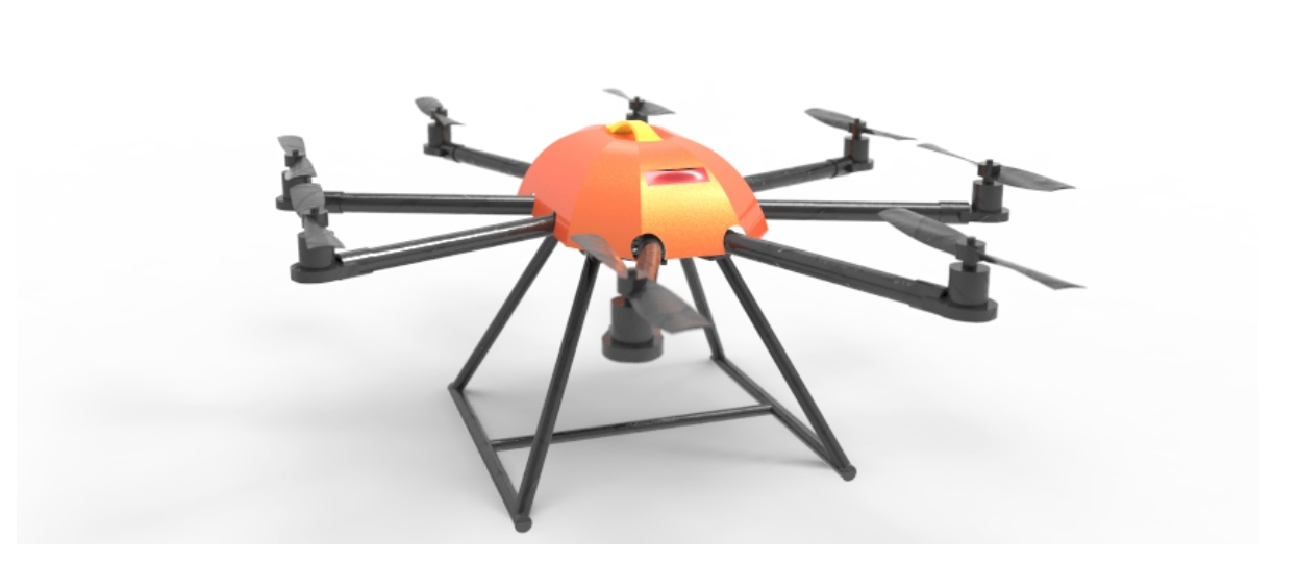
\includegraphics[keepaspectratio=true,scale=0.5]{figuras/keyshot1.eps}
    \caption{ Renderização do Projeto EmerVANT}
    \label{fig:keyshot1}
\end{figure}

O retângulo vermelho, presente na parte superior da estrutura do VANT, mostrado na figura 21, é a gaveta para retirada dos eletrodos do Desfibrilador Externo Automático, o local onde os eletrodos ficam guardados será passado para o usuário através do procedimento de instruções para a utilização do EmerVant. A central ficará responsável por dar todas as informações necessárias para a utilização do equipamento e atendimento.

\begin{figure}[H]
    \centering
      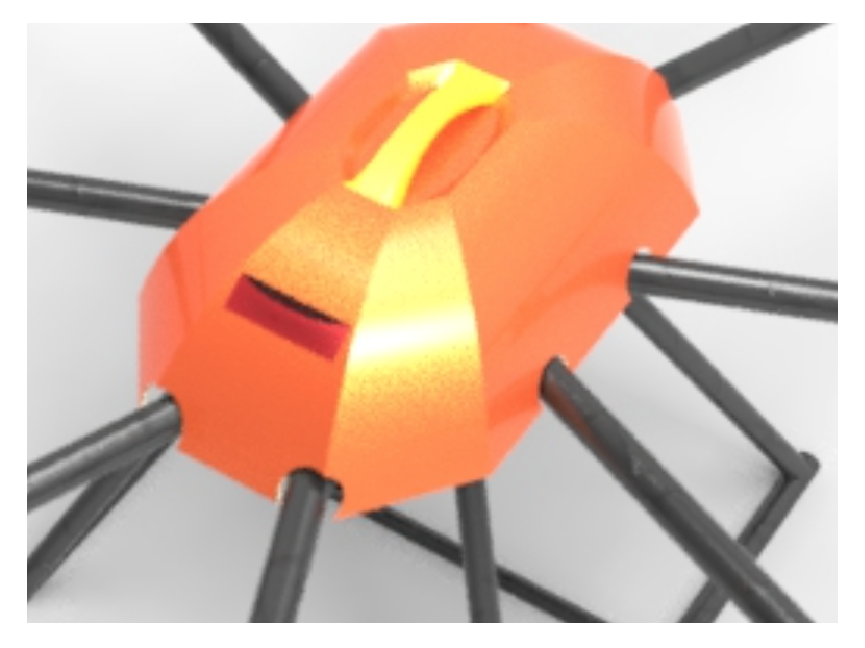
\includegraphics[keepaspectratio=true,scale=0.5]{figuras/keyshot2.eps}
    \caption{ Gaveta para eletrodos}
    \label{fig:keyshot2}
\end{figure}

\subsubsection{Análise de custos}

\indent \textbf{Frame central e trem de pouso}

Como definimos projetar alguns acessórios do VANT, como frame central, trem de pouso e a carcaça, foram levantados alguns estudos sobre como será projetado. O frame central e o trem de pouso, ambos serão projetados com fibra de carbono, pois se tratam de estruturas com características mais rígidas e resistentes para que possa suportar as tensões calculadas.

O preço do metro quadrado encontrado para esta fibra de carbono de pano liso está entre R\$150 e R\$200. Para realizar os custos de cada peça, atribuímos o valor de R\$200 o metro quadrado.

Todos os cálculos feitos a seguir são aproximações de comprimento dos componentes acima listados com uma margem de erro de 5\% para mais.

\begin{figure}[H]
    \centering
      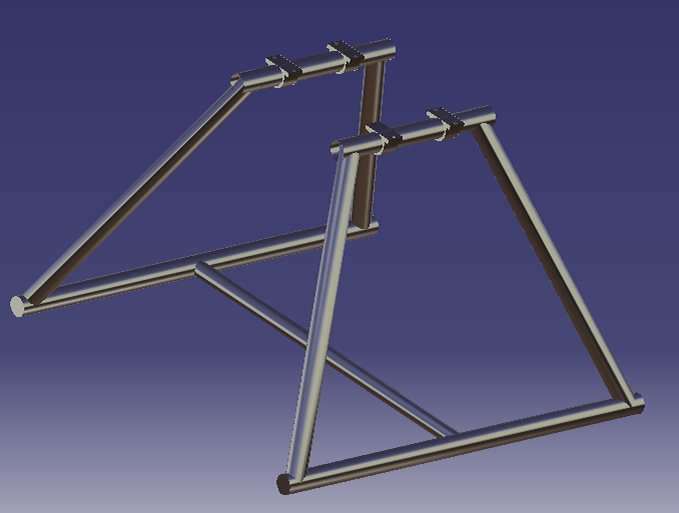
\includegraphics[keepaspectratio=true,scale=0.5]{figuras/frame_central.png}
    \caption{Trem de pouso CATIA}
    \label{fig:frame_central}
\end{figure}

Os tubos de fibra de carbono, que compõe o trem de pouso apresentado na figura \ref{fig:frame_central},
com 21 mm de diâmetro externo, 2 mm de espessura e 1m de comprimento custarão em torno de
R\$140 e R\$160 cada. O numero de tubos necessários para a construção do VANT serão de 8 devido
as varrições de comprimento de cada seção. Estas seções podem variar entre um comprimento de
251mm e 388mm.

De acordo com o preço de cada tubo, o preço total será de R\$1280. A junção destes será feita
por técnico mecânico industrial com valor de serviço de R\$20 (Guia do Estudante)\footnotemark a hora.

\footnotetext{http://guiadoestudante.abril.com.br/profissoes/engenharia-producao/automacao-industrial-684507.shtml}

Este técnico também elaborará a produção do Frame Central de acordo com os detalhes
especificados. Devido a esta peculiaridade a produção desta demorará em torno de 6 horas e as
junções das conexões das seções restantes terá tempo estimado de 16 horas, totalizando um total de
22h horas.

Portanto, o valor de número de horas a ser pagas a este técnico terá custo de no minimo
R\$440,00. Somando o preço total a ser pago para o número de tubos e horas trabalhadas, o valor total
a ser empregado nesta parte do projeto será de R\$1765,00.

\begin{table*}[!h]
\centering
    \caption{Custo de Fabricação das peças com Fibra de Carbono}
\begin{tabular}{|p{0.20\linewidth}|p{0.15\linewidth}|p{0.15\linewidth}|p{0.15\linewidth}|p{0.15\linewidth}|p{0.15\linewidth}|}
\hline

Peça & Preço& Quantidade& Horas Trabalhadas &HT x Hora técnico& Total\\ \hline
Frame Central &R\$ 22,50& 2 &3h x 2 = 6h& 6h x R\$20 = R\$120,00& R\$165,00 \\ \hline
Tubos (trem de Pouso)& R\$160,00& 8 &2h x 8 = 16h &16h x R\$20 = R\$320,00& R\$1600,00\\ \hline
\textbf{Total} & & & & & \textbf{R\$1765,00}\\ \hline

\end{tabular}
    \label{custos_carregador}
\end{table*}

\pagebreak
\indent \textbf{Carcaça}

Foi decidido que a carcaça do EmerVANT será feita através de uma impressora 3D
com o polímero ABS como material.

\indent \indent \textbf{Funcionamento da impressora 3D}

\begin{figure}[H]
    \centering
      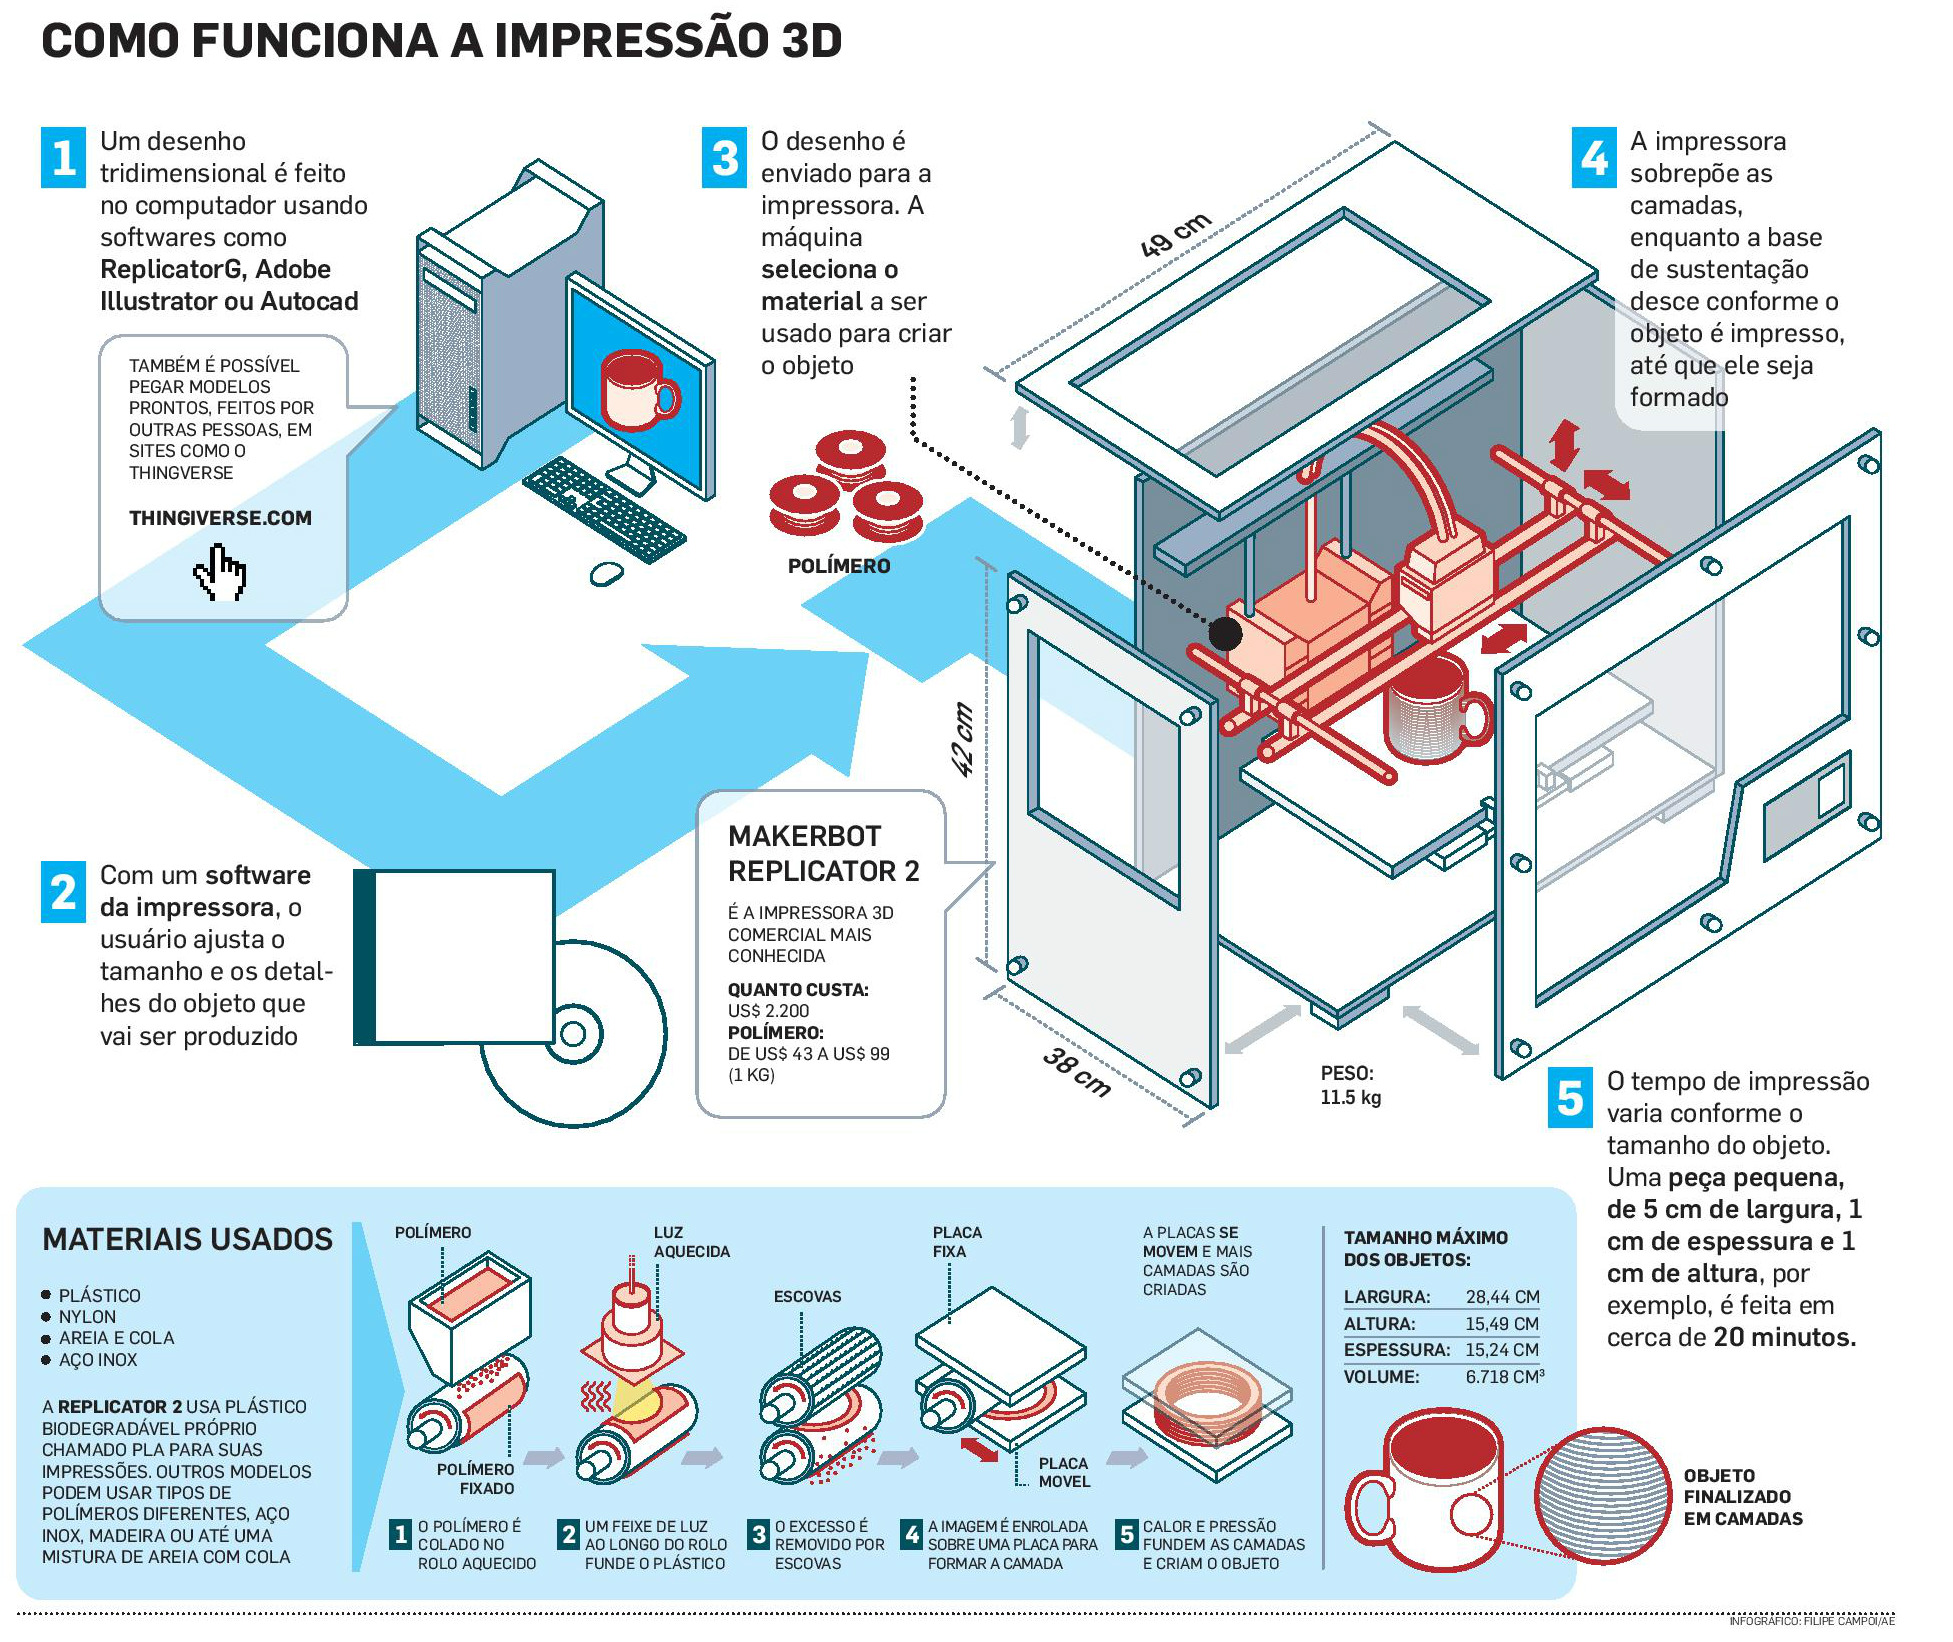
\includegraphics[keepaspectratio=true,scale=0.25]{figuras/impressao3D.jpg}
    \caption{Funcionamento de uma impressora 3D. Fonte: Fireprint}
    \label{fig:impressao3D}
\end{figure}

\footnotetext{http://www.graficafireprint.com.br/impressoras-3d/}
De acordo com o site da \textit{MakerBot}\footnotemark, as peças de filamento de plástico ABS são vendidas em quilograma, uma peça contendo um quilograma custa US\$48,00, como a carcaça do EmerVant tem aproximadamente 0,6363kg usando o polímero ABS, convém comprar somente uma  peça contendo um quilograma. Para ser enviada à Brasília as taxas de entrega resultam em US\$85,77, gerando um total de US\$133,77. Usando a cotação do dólar do dia 18/06/2015 as 17:24 de US\$3,0588, resultando assim R\$409,18.

O tempo para projetar a carcaça é de no mínimo 3 horas e o custo de um projetista atualmente no mercado é de aproximadamente R\$17,00 a hora resultando assim o custo de projeto em R\$51,00.

Foi feito um orçamento na empresa Grupo Alutech para fazer a confecção da carcaça do EmerVant usando polímero ABS na cor amarela custa no total com o frete R\$2145,00.

O custo total da carcaça do EmerVant somando projeto e material é R\$ 460,18. Se for contratada uma empresa para fazer o serviço, então o custo seria somente o de projeto e o da empresa, resultando em R\$2196,00.

\footnotetext{http://www.makerbot.com/search?q=ABS}

\indent \textbf{Braço, Hélice e Motor}

O motor, o braço e a hélice serão baseadas no VANT S1000 do fabricante DJI, o que
não será necessário projetar ambas as peças. No site \textit{Dronestore}\footnotemark é possível comprar o
conjunto motor, hélice e braço.

\footnotetext{http://www.dronestore.com.br/}

\begin{figure}[H]
    \centering
      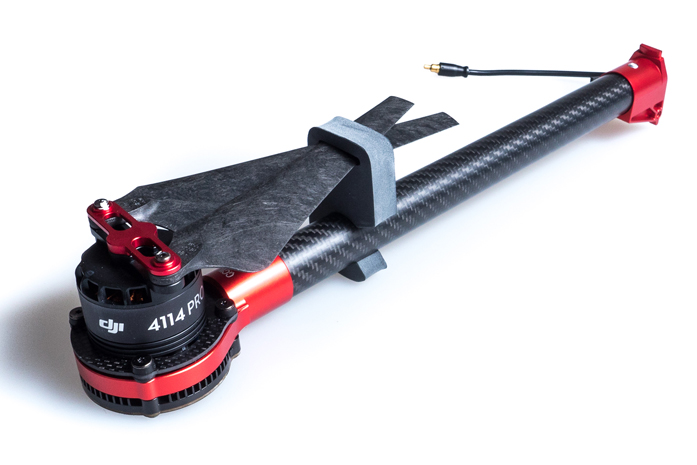
\includegraphics[keepaspectratio=true,scale=0.4]{figuras/braco_helice.jpg}
    \caption{Conjunto braço, motor e hélice. Fonte: \textit{Dronestore}}
    \label{fig:braco_helice}
\end{figure}

Conforme o verificado no site \textit{Dronestore}, o valor de um conjunto como acima, custa
R\$1654,00. Como são 8 braços, o valor total será de R\$13.232,00.

\indent \textbf{Desfibrilador e Reanimador Manual}

No caso do Desfibrilador Externo Automático (DEA), não será necessário fabricar um
para o projeto. Apenas será feito a compra de um DEA chamado \textit{HeartSine samaritan PAD
SAM 300P}. Conforme feito pesquisas para saber quanto custa, no site \textit{First Aid Product}\footnotemark, está
no preço de U\$1.600,00. Usando a cotação do dólar do dia 18/06/2015 as 17:24 de
US\$3,0588, o valor sai em R\$4.594,00.
\footnotetext{http://www.first-aid-product.com/}

No caso do Reanimador Manual, são 3 tipos de reanimador: Neonatal, Reanimador Infantil e Reanimador Adulto a partir dos 13 anos. R\$140,00 - cada unidade\footnotemark. 
Será realizado a compra do conjunto de Reanimadores da marca PROTEC\footnotemark.

\footnotetext{http://www.medicalfast.com.br/}
\begin{figure}[H]
    \centering
      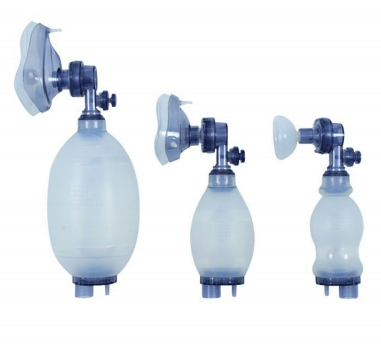
\includegraphics[keepaspectratio=true,scale=0.4]{figuras/reanimadores.png}
    \caption{Tipos de Reanimadores Manuais. Fonte: PROTEC}
\end{figure}

\footnotetext{http://www.protec.com.br/}
No Total, o conjunto de reanimadores custará R\$420,00.

\indent \textbf{Total}

\begin{table*}[!h]
\centering
    \caption{Custos totais da parte estrutural}
\begin{tabular}{|p{0.20\linewidth}|p{0.20\linewidth}|p{0.20\linewidth}|}
\hline

Peça &Quantidade& Preço\\ \hline
Tubos (Trem de pouso)&8 &R\$1600,00\\ \hline
Frame Central &2 &R\$165,00\\ \hline
Braço, hélice e motor &8 &R\$13.232,00\\ \hline
Desfibrilador &1 &R\$4.594,00\\ \hline
Reanimador &3 &R\$420,00\\ \hline
Total& &R\$20.011,00\\ \hline
\end{tabular}
\end{table*}

O conjunto estrutural do EmerVANT terá um valor minimo de R\$20.011,00, desconsiderando a parte controladora do VANT.
  
\subsection{Sistema de Controle do VANT}
  \subsubsection{Central de Atendimento}
A Central de Atendimento/ Estação Base do VANT, será um local, qual será responsável por controlar toda a operação de atuação do VANT, desde o atendimento da chamada, ao desenvolvimento do plano de voô do mesmo. É responsabilidade do controlador auxiliar no uso do desfibrilador em casos de emergência. Sendo que, tal Base, estará sempre acompanhando o atendimento ao paciente e monitorando o funcionamento do VANT, através da alta gama de sensores e câmeras espalhadas pelo equipamento.

Não há qualquer requerimento especificado para o uso do software de controle, logo um computador padrão com capacidade média de processamento é o suficiente para o uso do software, se vê a importância de destacar que o computador deve possuir uma placa de rede para acesso à internet. Para o computador, foi escolhido um processador Intel I5 e 8GB de memória RAM, com essas configurações é garantido desempenho suficiente com um preço não elevado.  

O atendente que controlará o VANT e atenderá os chamados deve ser um médico socorrista com capacidade de auxiliar o uso do desfibrilador por pessoas leigas. Como a central funcionará 24 horas por dia, se vê necessário o uso de uma rotação de funcionários, levando em conta uma carga horária de 8 horas por dia para cada atendente. Por ser um serviço essencial que não pode ser interrompido, cada atendente deve possuir um substituto hábil de plantão.

Tal Central de Atendimento/Base Estação, apresentará as seguintes características:

\begin{itemize}
  \item 01 - Equipe, composta por 02 pessoas capazes de operar os equipamentos e softwares da Estação Base e do VANT
  \item 02 - Computadores DELL – InspironSmall Desktop \cite{DELL}
  \item 01 Gerador de Energia a Gasolina Portátil \cite{Gerador}
\end{itemize}


\subsubsection{Controlador Pixhawk}
O módulo Pixhawk piloto automático é um sistema muito eficiente em tempo real de operação. 
O software pode ser atualizado com um bootloader USB (gerenciador de boot USB), que é um programa simples com a 
função de acessar o disco do computador e carregar o sistema operacional na memória para assumir o controle do 
equipamento.

Os benefícios do sistema Pixhawk incluem \textit{multithreading}, ou seja, a capacidade de servir mais de um usuário ao 
mesmo tempo, um ambiente de programação Unix/Linux capaz de gerar novas funções de piloto automático, como 
escrita de missões e comportamento de voo. \cite{pix}
 
O módulo Pixhawk flagship pode ser utilizado visando as novas opções de periféricos, como sensor digital de velocidade do ar, o suporte para um indicador LED externo multicor e um magnetômetro externo. Todos os periféricos são automaticamente detectados e configurados. \cite{pix}

\subsubsubsection{Especificações}

\textbf{Processador}
\begin{itemize}
	\item 32-bit ARM Cortex M4 com FPU
	\item 168 Mhz/256 KB RAM/2 MB Flash 
	\item 32-bit failsafe co-processor
\end{itemize}

\textbf{Sensores}
\begin{itemize}
\item MPU6000 com aceleração principal e giroscópio
\item ST Micro 16-bit giroscópio
\item ST Micro 14-bit acelerômetro /magnetmetro  MEAS barômetro
\end{itemize}

\textbf{Power}
\begin{itemize}
\item Controlador possui um diodo ideal com \textit{failover} automático.
\item Servo anteparo de alta potência (7V) e alta corrente de propensão.
\item Todas as saídas periféricas com \textit{over-current}, assim como todas as entradas ESC, possuem proteção.
\end{itemize}

\textbf{Interfaces}
\begin{itemize}
\item 5x UART com porta serial, 1 componente \textit{high-power}, 2x HW com controle de fluxo.
\item Spektrum DSM/DSM2/DSM-X entrada de satélite
\item \textit{Futaba} S.BUS entrada ( saída não implementada)
\item PPM sinal de soma
\item RSSI (PWM ou tensão) entrada
\item I2C, SPI, 2x CAN, USB
\item 3.3 e 6.6 ADC entradas
\end{itemize}

\textbf{Dimensions}
\begin{itemize}
\item Peso 38 g (1.3 oz)
\item Largura 50 mm (2.0”)
\item Altura 15.5 mm (.6”)
\item Comprimentob 81.5 mm (3.2”)
\end{itemize}

\begin{figure}[H]
	\centering
	  \includegraphics[keepaspectratio=true,scale=0.6]{figuras/pix1.eps}
	\caption{Visão geral da Pixhawk. Fonte \cite{pixhawk}}
	\label{fig:pix1}
\end{figure}

\begin{figure}[H]
	\centering
	  \includegraphics[keepaspectratio=true,scale=0.6]{figuras/pix2.eps}
	\caption{Entradas  de comunicação de dados  do Pixhawk. Fonte \cite{pixhawk}}
	\label{fig:pix2}
\end{figure}

\begin{figure}[H]
	\centering
	  \includegraphics[keepaspectratio=true,scale=0.6]{figuras/pix3.eps}
	\caption{Esquema da placa controladora Pixhawk. Fonte \cite{pixhawk}}
	\label{fig:pix3}
\end{figure}

\begin{figure}[H]
	\centering
	  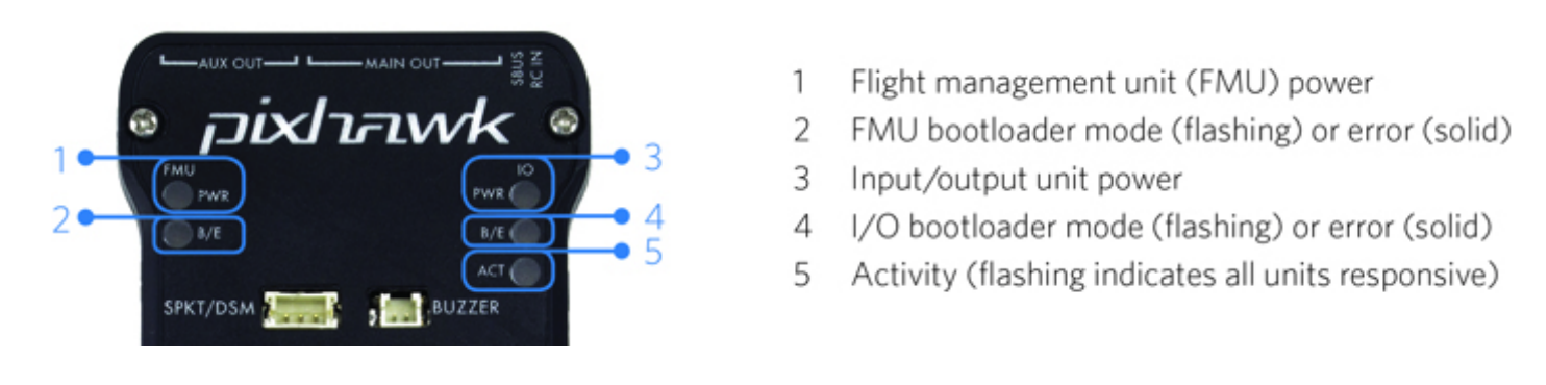
\includegraphics[keepaspectratio=true,scale=0.6]{figuras/pix4.eps}
	\caption{Esquema da placa controladora Pixhawk. Fonte \cite{pixhawk}}
	\label{fig:pix4}
\end{figure}

\begin{figure}[H]
	\centering
	  \includegraphics[keepaspectratio=true,scale=0.6]{figuras/pix5.eps}
	\caption{Esquema da placa controladora Pixhawk. Fonte \cite{pixhawk}}
	\label{fig:pix5}
\end{figure}

\begin{figure}[H]
	\centering
	  \includegraphics[keepaspectratio=true,scale=0.6]{figuras/pix6.eps}
	\caption{Esquema da plana controladora Pixhawk. Fonte \cite{pixhawk}}
	\label{fig:pix6}
\end{figure}


\subsubsection{Funcionamento do VANT}

Os VANT's por serem um tipo de veículo de pequeno porte e em conseqüência a miniaturização de seus componentes eletrônicos e seu barateamento, têm-se sua utilização gradativamente aumentada nas mais diversas áreas, como: vigilância, análise ambiental, missões militares e busca e salvamento de pessoas tanto em auto mar, como em áreas de pouco acesso. \cite{Branco}

O VANT projetado,será composto por um complexo sistema integrado, apresentando cinco sub-módulos principais  que trabalham em conjunto afim de obter uma alta plataforma de observação e atuação.

Sendo esses módulos, baseados em \cite{pastor}

\begin{itemize}
	\item Estrutura do VANT – Uma estrutura simples, leve, aerodinamicamente eficiente e com uma plataforma estável, capaz de oferecer uma otimizização na qualidade de voo do mesmo. 
	\item Controlador do VANT – Para realizar todo o processo de controle, comunicação externa e autonomia de voo do VANT, será utilizado o controlador PIXHAWK, da empresa 3D Robotcs, um sistema de computador concebido para coletar informações aerodinâmicas através de um conjunto de sensores(acelerômetros, giroscópios, magnetômetros, sensores de pressão, GPS, etc.), de modo a pilotar automaticamente o VANT.
	\item Caixa de Sensoriamento - Um conjunto de sensores compostos por câmeras de TV, sensores infravermelho, sensores térmicos, etc., para reunir informações que podem ser parcialmente processadas \textit{on-board}, pelo próprio controlador do VANT, ou transmitidas a uma base estação, para posterior análise.
	\item Estação Base – Uma equipe de chão, situada em uma região próxima a área de atuação do VANT, destinada a monitorar o desenvolvimento do voo, acompanhar e orientar o atendimento de emergência e eventualmente operar o VANT, caso ocorra alguma falha técnica. 
	\item Infraestrutura de Comunicação - Uma mistura de mecanismos, equipamentos e técnicas de comunicação (moldens de rádio,satcomm, links de microondas, etc.) que devem garantir um elo contínuo e estável entre o VANT e a estação de base. 
\end{itemize}


\begin{figure}[H]
	\centering
	  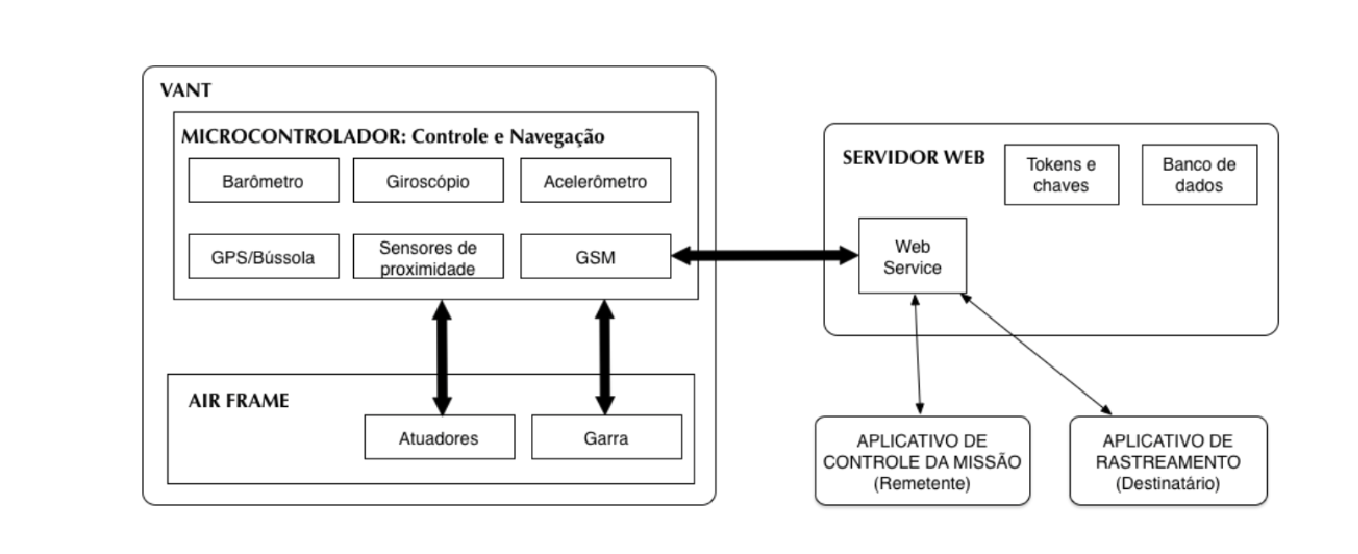
\includegraphics[keepaspectratio=true,scale=0.7]{figuras/diagrama.eps}
	\caption[Diagrama simplificado da comunicação do VANT com a Central.]{Diagrama simplificado da comunicação do VANT com a Central. Fonte \cite{Branco}}
	\label{fig:diagrama}
\end{figure}

A arquitetura de implementação do VANT utilizará microcontroladores, assim como sensores e módulos de transmissão de dados (Figura \ref{fig:diagrama}).
Os dados transmitidos entre o servidor na central de monitoramento, o VANT e os aplicativos (controle da missão e rastreador) seguirão um determinado padrão. Em caso de perda sinal, com a central de controle, o VANT será programado para que retorne automaticamente para a base de controle.

A Figura \ref{fig:esquemageral} mostra o esquema simplificado de montagem dos componetes do VANT.

\begin{figure}[H]
	\centering
	  \includegraphics[keepaspectratio=true,scale=0.6]{figuras/esquemageral.eps}
	\caption{Esquema de montagem do VANT. Fonte:\cite{esquematico}}
	\label{fig:esquemageral}
\end{figure}

\pagebreak

\subsubsection{Sistema de comunicação via rádio frequência}

Os sistemas de comunicação sem fio são baseados em campos eletromagnéticos, e são ondas que transportam energia de um ponto ao outro, isso possibilita que haja comunicação sem a necessidade de uma conexão física dos fios \cite{VALLE1}. 

Para que haja a propagação do sinal de radiofrequência (RF) é necessário que o sinal seja conduzido por um cabeamento condutor até uma antena que posteriormente irá irradiar através do ar os pulsos eletromagnéticos do sinal \cite{VALLE1}. 

A antena é um componente responsável por converter um sinal, do meio cabeado, em um sinal wireless (sem fio) e vice-versa. Os sinais irradiados no ar livre, em forma de ondas eletromagnéticas, propagam-se em linha reta e em todas as direções \cite{Rappaport2}. Com isso pode-se transmitir qualquer tipo de informação a um receptor remoto apenas utilizando a propagação dessas ondas eletromagnéticas.

\begin{figure}[H]
	\centering
	  \includegraphics[keepaspectratio=true,scale=0.6]{figuras/antena.eps}
	\caption{Transmissão radioelétrica de informação. Fonte: \cite{antena}}
	\label{fig:antena}
\end{figure}

\subsubsection{Radiofrequências}

O espectro eletromagnético da radiofrequência ocupa as frequências entre os 3 kHz e os 300 GHz. 

A figura \ref{fig:tabelafre} mostra as bandas de radiofrequência, o nome das respectivas e suas aplicações tradicionais.

\begin{figure}[H]
	\centering
	  \includegraphics[keepaspectratio=true,scale=0.6]{figuras/tabela.eps}
	\caption{Bandas de Radiofrequência. Fonte: \cite{tabela}}
	\label{fig:tabelafre}
\end{figure}

As ondas de radiofrequência de médias e baixas frequência (MB e ELF) possuem grandes comprimentos de onda, essa característica favorece a difração na atmosfera e garante que os obstáculos de grandes dimensões sejam contornados mais facilmente \cite{Rappaport2}.

Quanto maior a frequência menos é a capacidade de transmitir para distâncias muito longas ao nível da superfície terrestre \cite{VALLE1}. 

\begin{itemize}
	\item As ondas MF são as ondas utilizadas nas estações nacionais, permitindo difundir o som com maior qualidade, embora com menor alcance;
	\item As ondas LF são utilizadas nas estações de rádio que transmitem a nível mundial;
	\item As ondas ELF, que têm frequências extra baixas, são utilizadas quando tem-se grande obstáculos e necessita enviar uma informação. 
	\item As Ondas HF e VHF, possuem pequenos comprimentos de ondas, geralmente sofrendo múltiplas reflexões na ionosfera e na superfície terrestre, não conseguem acompanhar a curvatura da Terra. São utilizadas em comunicações que não exigem grande alcance, mas quando é exigida a alta qualidade de som e imagem.
	\item As Ondas UHF, SHF e EHF são utilizadas para comunicação com satélites, pois o seu comprimento de onda é muito pequeno e ele não sofre quase que refração nenhuma na atmosfera. 
\end{itemize} 

\subsubsection{Agência Nacional de Telecomunicações - ANATEL}

Para que seja criado um novo link utilizando radiofrequência é necessário consultar a ANATEL, pois ela é responsável por manter o controle de todas as frequências utilizadas nas telecomunicações, para garantir que não exista interferências nas transmissões.

\begin{figure}[H]
	\centering
	  \includegraphics[keepaspectratio=true,scale=0.6]{figuras/anatel.eps}
	\caption{Atribuição de faixas de frequências na ANATEL. Fonte: \cite{anatel}}
	\label{fig:tabela}
\end{figure}


Para poder ter acesso a um canal de frequência é necessário cumprir o regulamento de uso do espectro de radiofrequências. Resolução Nº 259 de 19 de abril de 2001(Em anexo ao relatório);

\subsubsection{Especificação do projeto da comunicação do VANT}

Para a comunicação será utilizado dois canais.

\begin{itemize}
	\item Um canal será responsável apenas pela comunicação dos dados referentes ao deslocamento, ele será para o controle do VANT, então será transmitido informações da trajetória que será seguida para o piloto automático e em caso de emergência o controle manual.
	\item O outro canal será para transmissão dos dados de vídeo e áudio.
\end{itemize}

\subsubsection{A comunicação e transmissão de dados }

O piloto automático guiará o VANT até a emergência. A central receberá a solicitação do veículo e com as orientações do local do acidente, ela irá mapear o percurso a ser seguido para chegar até o destino.  Essas informações referentes ao trajeto e coordenadas de GPS serão passadas de forma wireless serialmente para o sistema e controladores do VANT. Para que isso aconteça, eles estarão conectadas por um canal de comunicação de radiofrequência.

A central necessitará passar informações ao usuário referentes ao atendimento, também precisará ver o estado do paciente e ver se os procedimentos foram realizados conforme as instruções e as informações dos sinais vitais da vítima para entender a real situação dele. Com isso a central receberá um sinal de áudio e vídeo e o VANT receberá apena o sinal de áudio da central. 

\subsubsection{Projeto da comunicação do VANT}
A comunicação da central de atendimento e o VANT será através de um link de radiofrequência, será criado um canal na faixa das VLF (Very Low Frequency).

\begin{itemize}
	\item A escolha dessa faixa de operação VLF foi devido à grande facilidade de propagação desses tipos de onda;
	\item Grande possibilidade de contorno de obstáculos de grandes dimensões;
	\item Baixa suscetibilidade de sofrer interferências;
	\item Propaga-se usando a atmosfera;
	\item Menores chances de perder o link do canal;
	\item A faixa das ELE e VLF estão disponíveis no Brasil. De 0 a 8,5 KHz temos essas duas faixas.
	\item O Canal de comunicação do VANT será nessa faixa de 3KHz a 8,5KHz.
\end{itemize}

\pagebreak


\subsection{Comunicação do VANT}
  \subsubsection{Protocolo de Comunicação via Rádio Frequência}

O protocolo utilizado no link de rádio frequência criado será o MAVLink - \textit{Micro Air Vehicle Message Marshalling Library} - é uma biblioteca de comunicação para 
pequenas quantidades de dados entre aeronaves não tripuladas e estações de controle em terra. 
Permitindo o envio de pacotes de informações através de \textit{byte-level serialization} o que torna 
compatível com qualquer onda de radio.\cite{mavlink}

Uma vez que a área de atuação do EmerVant é a Esplanada dos Ministérios, 
definido na seção \ref{escopo} - Escopo, a viabilidade e eficiência na implantação desse protocolo é
extremamente alta. Aonde o sinal emissor será posicionado na torre de TV cobrindo toda a 
área de atuação com um boa qualidade de sinal. 

\subsubsection{Especificação do Projeto da Comunicação do Vant}

A comunicação entre a central de atendimento, responsável por receber a chamada de emergência, e a central de controle, responsável pelo controle, comando e monitoramento do VANT, ocorrerá da seguinte forma:

\begin{itemize}
  \item A central de atendimento recebe a chamada de emergência.
  \item Verifica a necessidade de enviar o VANT. Analisando o tempo hábil para a chegada da ambulância.
  \item Caso necessário, a ambulância  ligará para a central de controle, para que a mesma envie o VANT para o local indicado.
  \item A partir da decolagem do VANT, a comunicação passa a ocorrer via RF(radiofreqüência) com a central de controle.
  \item Quando o VANT chegar ao local, o controlador instrui o usuário à usar o desfibrilador na vitima, se necessário. Tal comunicação é feita por RF.
  \item Após o atendimento, a ambulância que já terá se dirigido ao local de atendimento, para a finalização do atendimento e o encaminhamento da vitima para o hospital, ela recolherá o VANT.
 
\end{itemize}

\begin{itemize}
 \item Piloto automático guiará o VANT até a emergência: 

  A central receberá a solicitação do veículo e com as orientações do local do acidente, ela irá mapear o percurso a ser seguido para chegar até o destino.  Essas informações referentes ao trajeto e coordenadas de GPS serão passadas de forma wireless serialmente para o sistema e controladores do VANT. Para que isso aconteça, eles estarão conectadas por um canal de comunicação de radiofrequência. 

  \item Comunicação e transmissão de dados:

   A central necessitará passar informações ao usuário referentes ao atendimento, também precisará ver o estado do paciente e ver se os procedimentos foram realizados conforme as instruções e as informações dos sinais vitais da vítima para entender a real situação dele. 
\end{itemize}
\subsubsubsection{Comunicação com o Pixhawk}
O controle e configura\c{c}\~ao do voo do VANT \'e gerenciado pelo \textit{Ground Control Station}, em português, 
esta\c{c}\~ao de controle em solo. Inicialmente seria desenvolvido um sistema que atendesse os requisitos levantados no Documento
de Visão do Projeto (em anexo), todavia com a pesquisa de sistemas existentes concorrentes optou-se por utilizar o \textit{software Mission Planner}. 
Devido à facilidade na customização e a compatibilidade com a placa controladora adotada 
pelo projeto, Pixhawk, esse sistema é mantido pelo projeto \textit{open-source  APM autopilot}.\cite{gcs}

Foram analisados os seguintes \textit{softwares} e essa análise pode ser vista na Figura \ref{fig:gcstable}: 

\begin{itemize}
  \item QGroundControl
  \item Mission Planner
  \item APMPlanner
\end{itemize}

\begin{figure}[H]
    \centering
      \includegraphics[keepaspectratio=true,scale=0.45]{figuras/gcstable.eps}
    \caption{Resultado da análise dos softwares de GCS.}
    \label{fig:gcstable}
\end{figure}

\pagebreak
Pela Figura \ref{fig:gcstable}, pode-se perceber que o software Mission Planner é a melhor solução para o gerênciamento do VANT. Uma vez que o projeto está sob uma licença aonde é permitido o uso para comercialização, este será utilizado com GCS do VANT.

Com a utilização do \textit{GCS Mission Planner}, o processo da operação de socorro é automatizado. 
Uma vez que, com a aplicação é possível a criação de planos de voos. 
A figura \ref{fig:planovoo} mostra um exemplo de plano de voo. 
Nesse plano, o VANT decola do ponto \textit{Home}, em seguida é direcionado até ao ponto 2 e depois 
se desloca ao ponto 3 e retorna ao ponto inicial.

\begin{figure}[H]
    \centering
	    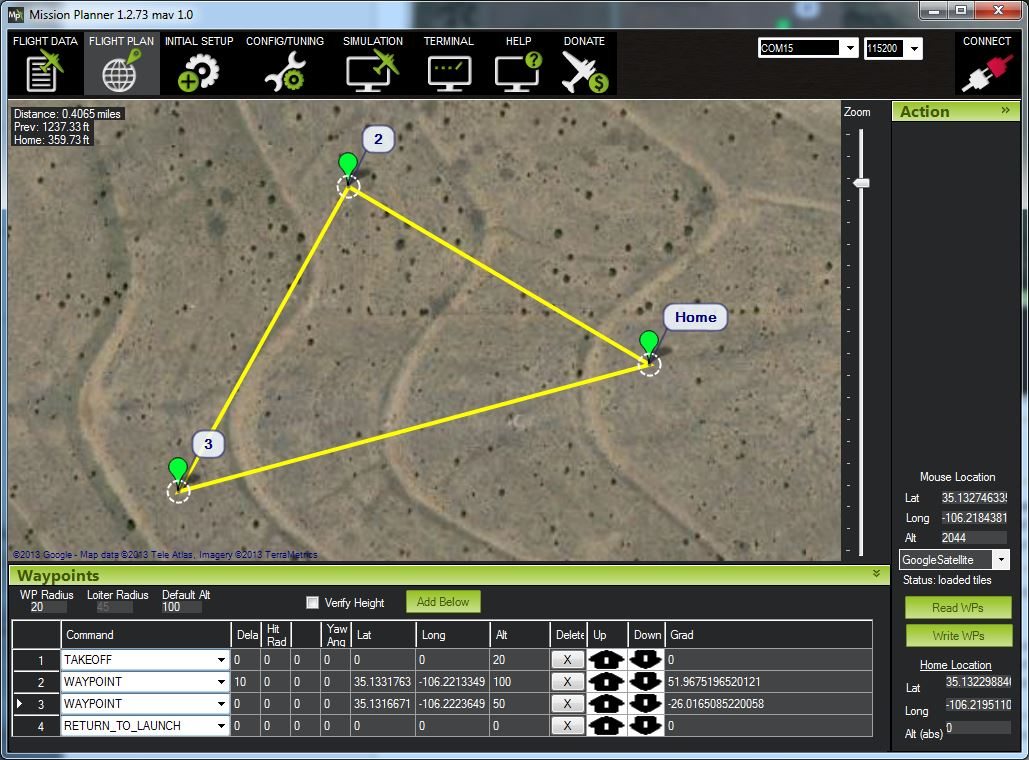
\includegraphics[keepaspectratio=true,scale=0.5]{figuras/planovoo.eps}
    \caption{Exemplo de missão da GCS. Fonte: Software \textit{Mission Planner}}
    \label{fig:planovoo}
\end{figure}


Os locais onde deve-se passar, ou pousar, ou executar um comando são definidos através das coordenadas de longitude e latitude. Assim quando ocorrer uma emergência, a equipe de controle, com o auxílio da API Google Maps integrada com o GCS, apontará as coordenadas aonde o VANT deve pousar para executar o socorro. 
A figura \ref{fig:esplanada} mostra uma missão na Esplanada dos Ministérios.

\begin{figure}[H]
    \centering
	    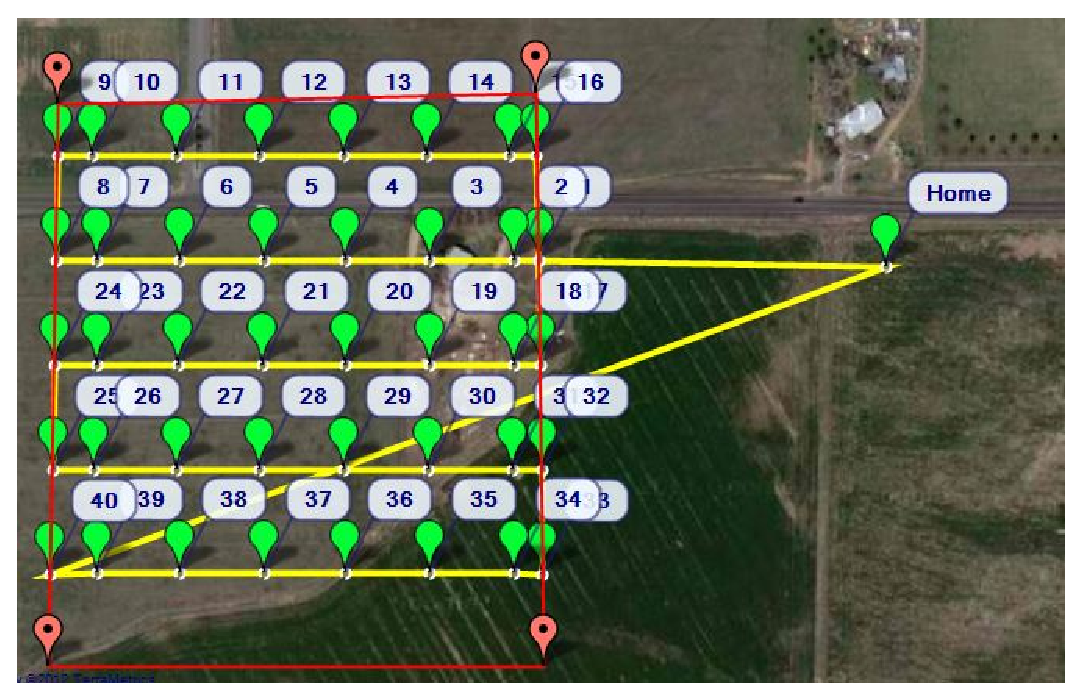
\includegraphics[keepaspectratio=true,scale=0.8]{figuras/esplanada.eps}
    \caption{Simulação feita na Esplanada. Fonte: Software \textit{Mission Planner}}
    \label{fig:esplanada}
\end{figure}

A plataforma a ser utilizado será o Microsoft Windows devido à grande utilização no Serviço Público, 
além de oferecer maior compatibilidade com os recursos utilizados, obedecendo, por exemplo, os requisitos
do sistema de comunicação com o controlador, o Mission Planner. 

\subsubsubsection{Protocolo de erros}
	
Para um funcionamento seguro é necessário ter em mente que podem vir a existir condições adversas as planejadas. Tendo isso em vista foi estabelecido um protocolo de erros para situações que podem vir a ocorrer durante um voo do VANT.

\begin{itemize}
 \item Perda de sinal: Em caso de perda de sinal o VANT deverá retornar a seu ponto de origem imediatamente.
 
 \item Bateria fraca: Ao chegar em 25\% restante de bateria o VANT irá retornar para a central imediatamente.

 \item Perda de potência: Em caso de perda de potência por parte do motor, o VANT procurará um local para pousar imediatamente.

\end{itemize}

\subsubsubsection{Comunicação do usuário com o VANT}
Nessa subseção é tratada a comunicação da central com o VANT e do cidadão com o VANT.
Nessa comunicação alguns passos devem ser seguidos, são eles:

\subsubsubsection{Processo de atendimento adotado}
Mediante análise do sistema de atendimento de urgências e classificação da situação-problema adotado em uma capital brasileira, além de questões de segurança de uso do VANT, identificou-se a necessidade de um protocolo de atendimento para verificar a viabilidade do atendimento pelo VANT ou por uma viatura comum de atendimento de urgência.
Ao receber a solicitação de socorro, o atendente avalia a situação da emergência, como identificação do paciente, localização do chamado e origem e natureza do solicitante. Em posse dessas informações, verifica-se a necessidade e disponibilidade de uma viatura para atendimento solicitado.

% image

É de competência do médico regulador avaliar qual o melhor recurso para o paciente, ou seja, sua decisão poderá ser a de orientar o solicitante a procurar uma unidade de saúde ou, nos casos necessários, enviar ao local uma Unidade de Suporte Básico, com auxiliar de enfermagem e condutor socorrista, ou uma Unidade de Suporte Avançado, a UTI móvel, com médico e enfermeiro.
A atividade do médico regulador envolve o exercício da Telemedicina, que se dá através da gravação contínua das comunicações, do correto preenchimento das fichas


médicas de regulação e do seguimento de protocolos institucionais normatizados que definam os passos e as bases para sua decisão, sempre julgando a necessidade do envio da melhor resposta e do melhor recurso às diversas solicitações. Nos casos em que o médico regulador julgar desnecessário o envio de uma equipe ao local para atendimento às solicitações, o mesmo deve explicar sua decisão e esclarecer ao demandante do socorro quanto a outras medidas a serem adotadas, por meio de orientação ou conselho médico, que permita ao solicitante assumir cuidados ou buscá-los em local definido pelo médico regulador.

Para garantir um funcionamento adequado do modelo de regulação referenciado, algumas tecnologias estão sendo incorporadas à central de regulação médica das urgências como o sistema de rastreamento dos veículos através de GPS (Global Positioning System) e ainda a transmissão de dados para o interior das ambulâncias e vice-versa.
Estas ferramentas oferecem informações que servem para auxiliar na decisão gestora do regulador médico, uma vez que atuam sobre dois dos grandes nós críticos do atendimento pré-hospitalar móvel, a comunicação qualificada com as equipes de atendimento e a diminuição do tempo resposta.

\subsubsubsection{Avaliação multifatorial do grau de urgência}

O grau de urgência é diretamente proporcional à gravidade, à quantidade de recursos necessários para atender o caso e à pressão social presente na cena do atendimento, e inversamente proporcional ao tempo necessário para iniciar o tratamento. Levando-se em conta esta razão matemática, temos a seguinte fórmula.

% image

\begin{description}
  \item[Gravidade] \hfill \\
  É perfeitamente possível quantificar a gravidade do caso pelo telefone, por meio de perguntas objetivas dirigidas diretamente ao paciente ou à pessoa que ligou solicitando ajuda, utilizando uma semiologia que é definida e abordada nos protocolos específicos.
 \item[Tempo] \hfill \\
 Tratamos aqui de utilizar o conhecimento dos intervalos de tempo aceitáveis entre o início dos sintomas e o início do tratamento. Quanto menor o tempo exigido, maior a urgência.
 \item[Recursos necessários] \hfill \\
 Quanto maior for a necessidade de recursos envolvidos no atendimento inicial e no tratamento definitivo, maior será a urgência. Este subfator é o que mais influi na decisão de transferir o paciente.
  \item[Valor Social] \hfill \\
 A pressão social que envolve o atendimento inicial pode muitas vezes justificar o aumento do grau de urgência de um caso simples. Este fator não pode ser negligenciado, pois muitas vezes uma comoção social no local do atendimento pode dificultar a prestação de socorro.
\end{description}

\subsubsubsection{Classificação das urgências}

Com o objetivo de facilitar o estabelecimento de prioridades entre os diferentes casos de urgência, podemos classificar, didaticamente, as solicitações de socorro da seguinte forma:

% image tabela

Como o veículo aéreo não tripulado se direciona apenas para atendimento de casos de extrema urgência com a impossibilidade da chegada de uma Unidade de Atendimento Básico em tem hábil. O VANT pode ser acionado apenas em casos com classificação 1 (um) de urgência, em que o tempo é primordial para atendimento e que haja algum bloqueio da ambulância.

Avaliando a setorização da Central de Atendimento do Serviço Móvel de Urgência, acontecerá a transferência de comunicação para um setor especializado no controle dos VANT’s que se localizará no mesmo local físico que a Central de Atendimento no Batalhão do Corpo de Bombeiros Militar da Esplanada dos Ministérios próximo ao Palácio do Planalto na Esplanada dos Ministérios em Brasília-DF.

O VANT estará posicionado nessa mesma base, em que um técnico colocará o veículo disponível em local aberto, confirmando as corretas informações dos sensores a central. Após a decolagem o veículo será monitorado apenas pelo software e recursos embutidos. A central pode avaliar toda a situação através de sensores, vídeo e áudio, avaliando assim a correta localização e a emergência. 

Após a conferência, o veículo poderá solicitar espaço para pouso seguro, alertando pessoas próximas para continuação do atendimento. Levando o mesmo para perto do local de emergência e posicionando o sensor no dedo indicador do paciente, averiguando a situação do mesmo identificando se o paciente sofre parada cardíaca ou respiratória.

Caso a situação não trate das doenças supracitadas, observa-se a situação por áudio e vídeo, estabelecendo protocolos de primeiros socorros, até a chegada da Unidade Móvel para o atendimento e recolhimento do veículo.

Entretanto, ao verificar a utilidade do VANT em tal atendimento, a comunicação com um terceiro torna-se essencial para continuação do socorro, por meio de áudio e visualização do paciente pela central. De modo que o atendente especializado possa instruir corretamente terceiros no posicionamento dos sensores do desfibrilador ou da bomba respiratória e os demais passos, como afastamento de pessoas do paciente ou o uso devido da bomba respiratória.

No caso do uso do desfibrilador, por ser um aparelho eletrônico portátil e automático que diagnostica as, potencialmente letais, arritmias cardíacas de fibrilação ventricular e taquicardia ventricular em um paciente. Capaz também de trata-las, através da desfibrilação, uma aplicação de corrente elétrica que para a arritmia, fazendo com que o coração retome o ciclo cardíaco normal.

Já no caso de parada respiratória, as instruções para utilização de Respiração Artificial Instrumental serão passadas e observadas pelo atendente da central. De modo a normalizar a ventilação por via aérea.

A central pode solicitar, via áudio, que o terceiro que auxiliou no atendimento aguarde no local até a chegada da viatura a fim de prevenir outros casos.

\subsubsection{Custos}
  
  Para a parte de comunicação o custo calculado trata-se das modificações a serem realizadas no
  \textit{Mission Planner}, essas modificações podem ser vistas no documento de visão que está
  em anexo.
  
  Dadas as modificações necessárias, para a realização das mesmas, foi definido um planejamento, usando o \textit{Scrum} que
  é uma metodologia ágil e que traz conceitos temporais que serão utilizados nas modificações do \textit{Mission Planner}. 
  
  Dentre os conceitos provenientes de \citeonline{scrum} que serão utilizados no projeto temos as seguintes definições:

  \begin{itemize}
  \item \textit{Release} – Entrega das manutenções planejadas. No projeto de manutenção do \textit{Mission Planner} será após um mês do começo das modificações;
  \item \textit{Sprint} – Ciclo menor de tempo. No projeto de manutenção do \textit{Mission Planner}, possuirá duas semanas de duração.
  \end{itemize}

  \textbf{Planejamento}
   \begin{itemize}
      \item 1ª \textit{Sprint}
	\subitem Retirar função de doar para o projeto;
	\subitem Traduzir menus, instruções e comandos;
	\subitem Criar funcionalidades de \textit{login}.	
      \item 2ª \textit{Sprint}
      \subitem Criar funcionalidade de receber dados do paciente.
      \subitem Adicionar funcionalidade de observação por câmera e comunicação;
      \subitem Definir perfis de acesso e configuração.
  \end{itemize}

 \textbf{Cálculo dos custos}
 
 Para definir os custos, foi definido que cada atividade deverá passar por quatro áreas: 
\begin{itemize}
 \item Requisitos;
\item Desenvolvimento;
\item Teste;
\item Implantação.
\end{itemize}

   Foi definido que a fábrica que realizará a manutenção possuirá três funcionários para cada uma das áreas descritas. 
   Foram definidos os seguintes salários (por hora), baseado no site Info Abril\footnotemark para os funcionários dessas áreas:
\footnotetext{http://info.abril.com.br/carreira/salarios/}
\begin{itemize}
   \item Analista de Requisitos – R\$ 91,50
\item Desenvolvedor – R\$ 53,20
\item Analista de Teste –R\$ 58,80
\item Infraestrutura – R\$ 63,00
\end{itemize}

Sendo assim, tendo em mente que serão duas \textit{sprints} de duas semanas cada, 
e que por dia cada funcionário trabalha 8 horas, temos como custo final o valor de R\$ 63960,00,
conforme detalhamento na figura \ref{fig:custos_software}.
 
 \begin{figure}[H]
    \centering
	    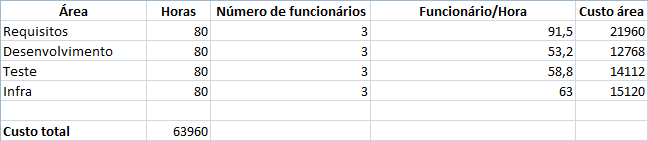
\includegraphics[keepaspectratio=true,scale=0.8]{figuras/custos_software.png}
    \caption{Custos de modificações no \texttt{Mission Planner}}
    \label{fig:custos_software}
\end{figure}

Algo que também deve ser levado em conta é que pode vir a existir a necessidade de manutenção, seja esta corretiva ou evolutiva, 
sendo assim deve ser levado em conta um possível gasto extra além do estabelecido.


\subsection{Equipamentos de socorro}
  Nessa seção estão descritos os equipamentos a serem levados no EmerVant.
  \subsubsection{Desfibrilador}

A escolha do desfibrilador, para ser carregado no VANT foi realizada visto que:

\begin{citacao}
foi documentada uma taxa de 
sobrevivência entre vítimas de parada cardíaca com fibrilação ventricular confirmada acima de 90\% quando a desfibrilação é atingida
dentro do primeiro minuto de colapso. As taxas de sobrevivência declinam 7 a 10\% a cada minuto em que a desfibrilação
é atrasada, de modo que uma vítima de parada cardíaca sem desfibrilação por 12 minutos tem apenas 2 a 5\%
de chance de sobrevivência.\cite{1}
\end{citacao}

O objetivo em realizar a Reanimação Cárdio-Pulmonar (RCP) é prover oxigênio ao cérebro e coração até que
o tratamento adequado restaure os batimentos cardíacos normais, ou que permita o tempo necessário para a 
chegada de uma equipe de socorro de Suporte Avançado de Vida (SAV). Quando o início da RCP for retardado, 
a chance de sobrevida é prejudicada e o córtex cerebral (o tecido mais susceptível à lesão por baixa de 
oxigênio no sangue) sofre danos irreversíveis,resultando em morte ou seqüelas neurológica severa e permanente. \cite{2}

O desfibrilador externo automático (DEA) por ser portátil e automático, torna a possível utilização por 
pessoas sem formação médica, visto que ele possui um computador embutido que verifica o ritmo cardíaco da 
pessoa e calcula se a desfibrilação se faz necessária, mostrando um comando para a pessoa acionar o botão, de 
modo a liberar a carga no peito da vitima.\cite{3}. O diagrama de bloco mostrado na Figura \ref{fig:dea}, mostra todo o funcionamento do DEA.

\begin{figure}[H]
	\centering
	  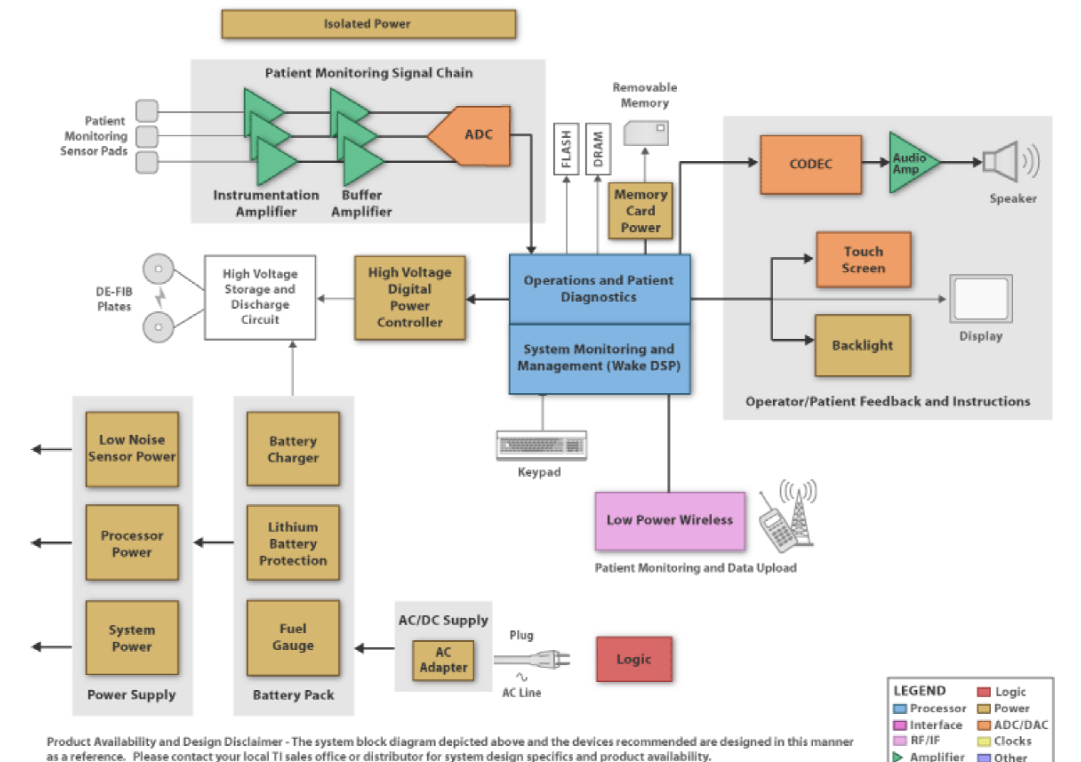
\includegraphics[keepaspectratio=true,scale=0.4]{figuras/dea.eps}
	\caption{Diagrama de bloco do desfribilador (DEA). Fonte: \cite{bloco}}
	\label{fig:dea}
\end{figure}

O desfibrilador, como demonstrado na Figura \ref{fig:dea}, consiste de uma fonte  de alimentação que 
fornece uma tensão regulada aos circuitos de controle e de interface do equipamento, além de fornecer uma carga.

A principal hipótese pela qual o choque elétrico desfibrilatório termina com a fibrilação ventricular (FV) se
baseia na despolarização de uma determinada massa crítica miocárdica, tornando-a temporariamente inexcitável, e
assim extinguindo as frentes de onda de excitação causadas pela manutenção da FV, de modo a permitir o 
restabelecimento do padrão normal de excitação e propagação elétrica (ZIPES et al., 1975 apud \citeonline{4}).

A figura \ref{fig:circuitodea} mostra todo o circuito eletrônico do DEA.

\begin{figure}[H]
	\centering
		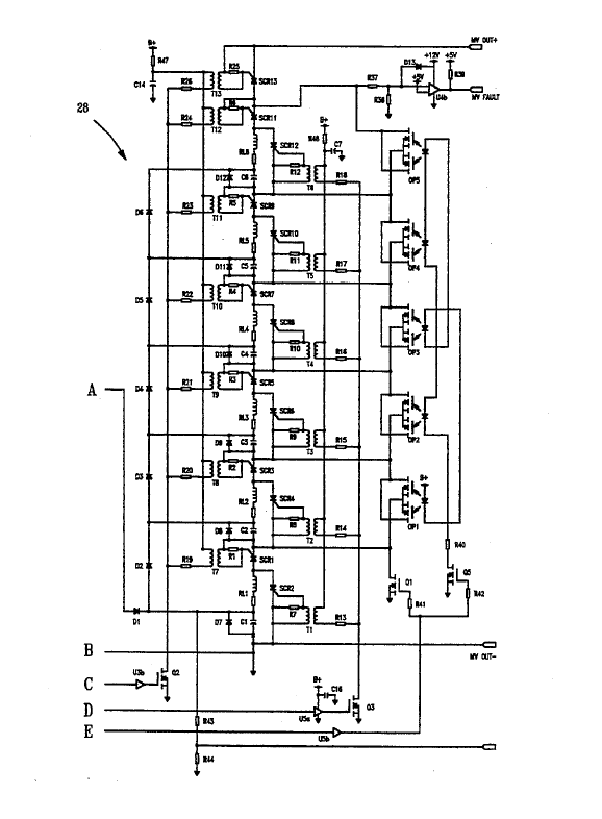
\includegraphics[keepaspectratio=true,scale=1.2,angle=-90]{figuras/circuitodea.eps}
	\caption{Circuito elétrico DEA. Fonte: \cite{dea}}
	\label{fig:circuitodea}
\end{figure}

\subsubsection{Reanimador Manual}
Para atendimento em urgência, o Reanimador Manual (RM), possibilita eficiente ventilação com ar, sendo este balão auto inflável de vinil.

Um dos recursos a ser utilizado no VANT é o RM, sendo que este produto engloba três categorias, o reanimador recém-nato, infantil e adulto. No projeto serão utilizadas as dimensões do RM infantil e adulto como referência, mas no VANT será utilizado um adaptador com velcro, viabilizando a adequação de cada reanimador, independentes de suas dimensões dentro da margem de tolerância estabelecida.

O RM é usado de acordo com o peso da vítima, se esta tiver menos de 10 kg, o RM a ser designado será o recém-nato, já o RM Infantil é voltado para aqueles entre 10 e 30 Kg. O RM adulto será aplicado a vítimas com 30 Kg ou mais.

Valores utilizados como peso, capacidade do balão entre outros, foram provenientes de informações referentes ao RM da marca Oxigel.

\begin{itemize}
	\item Características
\end{itemize}

\begin{table}[H]
\begin{tabular}{|l|l|l|l|}
\hline
\multicolumn{1}{|c|}{Reanimador} & Capacidade do Balão & Peso & Conexão \\ \hline
Adulto                           & 1200ml              & 410g & 22x15mm \\ \hline
Infantil                         & 500ml               & 210g & 22x15mm \\ \hline
\end{tabular}
\end{table}


\begin{itemize}
	\item Dimensionamento
\end{itemize}

\begin{table}[H]
\begin{tabular}{|l|l|l|l|}
\hline
\multicolumn{1}{|c|}{Reanimador} & Altura & Comprimento & Largura \\ \hline
Adulto                           & 14cm   & 38cm        & 18cm    \\ \hline
Infantil                         & 10cm   & 33cm        & 18cm    \\ \hline
\end{tabular}
\end{table}


\begin{figure}[H]
	\centering
	  \includegraphics[keepaspectratio=true,scale=0.6]{figuras/animadoradulto.eps}
	\caption{Reanimador Manual Adulto.}
	\label{fig:animadoradulto}
\end{figure}

\begin{figure}[H]
	\centering
	  \includegraphics[keepaspectratio=true,scale=0.6]{figuras/animadorinfatil.eps}
	\caption{ Reanimador Manual Infantil.}
	\label{fig:animadorinfatil}
\end{figure}



 
\subsection{Sistema de Fornecimento de Energia}
  
Para que o um veículo aéreo não tripulado funcione de forma completa, é necessário definir um sistema de fornecimento de energia eficiente, para que o mesmo consiga suprir todas as necessidades dos sistemas que terão funções de controle e comando.

\subsubsection{Bateria}

Uma bateria é um dispositivo capaz de armazenar energia química e transformá-la em energia elétrica. A bateria é entendida geralmente como algo que possui duas ou mais células elétricas individuais, e existem dois tipos básicos de células: primária e secundária \cite{gibbs}. As primárias, identificadas como células normais, não são recarregáveis e devem ser descartadas quando esgotadas. Já as secundárias, são recarregáveis, como a bateria do tipo polímero de lítio, que foi a escolhida para atuar neste projeto, e será apresentada posteriormente. 

Para determinar a escolha da bateria utilizada em qualquer projeto, é importante fazer a análise  da energia armazenada na bateria e a variação de descarga ao ser utilizada, e para calcular a energia armazenada, deve-se conhecer a tensão (V) e sua capacidade de descarga de corrente no tempo (Ah), utilizando a equação a seguir: \cite{peixoto}

$Energia(Wh)= Tensão(V)*Capacidade(Ah)$

Onde tensão ou diferença de potencial (DDP), é a diferença de potencial elétrico entre dois pontos ou a diferença em energia elétrica potencial por unidade de carga elétrica entre dois pontos, e sua unidade de medida é o Volt. E Capacidade (amp-hora ou mA-h) é a transferência de carga elétrica através de uma corrente estável de um ampere no período de uma hora \cite{gibbs}.

Além disso, deve-se também conhecer a densidade de energia (relação entre quantidade de energia por unidade de massa ou Volume), Resistência interna, voltagem, peso, viabilidade econômica e disponibilidade no mercado.


\subsubsection{Atuação do circuito na bateria}

O diagrama da figura \ref{fig:esquemabateria}, demonstra funciona o sistema de alimentação do circuito elétrico do VANT. É possível identificar a bateria principal (batt), ela é ligada a porta de alimentação do modulo de potência 3DR Pixhawk, que foi usado pois a bateria que está sendo usada necessita devido suas especificações. Posteriormente tudo é ligado a uma placa de distribuição de potência (PDB), onde ela é a responsável para suprir a necessidade do sistema, ela que alimentará a controladora Pixhawk com seus periféricos e mandará energia suficiente para suprir a corrente exigida dos escs para o funcionamento dos motores. Por segurança, há uma segunda fonte de alimentação, uma fonte de 5V (BEC), ela é para casos onde houver uma falha na fonte primária, dessa forma ela será automaticamente ativada para evitar possíveis falhas \cite{pix}.

\begin{figure}[H]
    \centering
	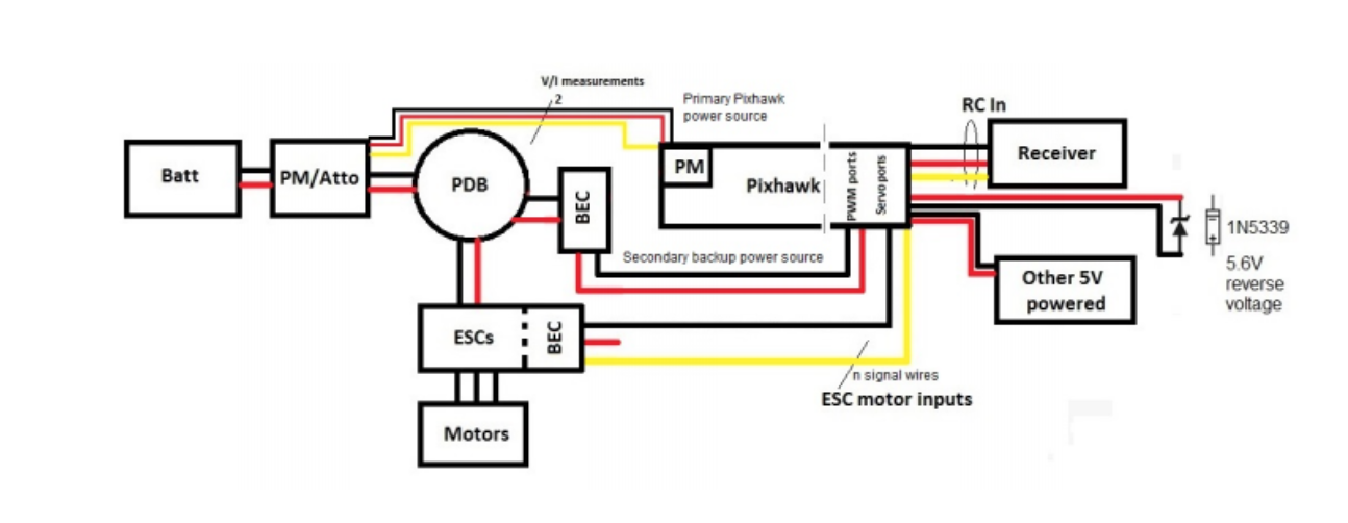
\includegraphics[keepaspectratio=true,scale=0.6]{figuras/esquemabateria.eps}
    \caption{Diagrama de blocos da bateria ligada ao controlador. Fonte: \cite{pixhawk}}
    \label{fig:esquemabateria}
\end{figure}


\subsubsection{Bateria de polímeros de Lítio (Li-Polymer)}

Baterias de polímeros de Lítio (LiPo) são aquelas que contem seus eletrólitos retidos em um polímero sólido, 
composta por várias células secundárias finas idênticas ligadas em paralelo, o que aumenta sua capacidade de 
descarga, sendo essencial que ela opere em uma faixa entre sua voltagem, não excedendo nem diminuindo muito, para perfeito funcionamento. \cite{gibbs}

As células de lítio-polímero são feitas de três componentes principais: um catodo (placa positiva), um anodo 
(placa negativa) e um separador. O catodo e o anodo são feitos principalmente de lítio, já o separador é feito 
de folhas rígidas de polímero banhadas em eletrólito. \cite{gibbs}

São flexíveis e oferecem leveza, já que não se faz necessário uma camada metálica externa como as baterias de 
Lítio-Íon, e podem ser facilmente moldadas para diversas aplicações. Também possuem uma resistência interna 
baixa que se adequa bem as altas taxas de descargas. \cite{costa}. Usada comercialmente desde 1999 as baterias 
de polímeros de Lítio possuem densidade de energia em torno de 100 e 130 Wh/kg, ou seja, quantidade de energia 
por volume relativamente alta, muito parecida com as baterias de Lítio-Íon. Com isso o fator mais importante para
análise é a tolerância para a sobrecarga, nas baterias de Lítio-polímero essa tolerância é maior, evitando um 
excesso de energia concentrado na bateria que ocasionaria a perda de rendimento ou até a perda total da bateria.
\cite{costa}

\subsubsubsection{Características bateria LiPo 6s}

O funcionamento básico da célula de bateria do tipo LiPo consiste em eletrólitos de sais de lítio retidos
em um polímero sólido com óxido de polietileno e o poliacrilonitrilo ao invés de solventes tornando-as
adaptáveis a diferentes formatos e permitindo altas taxas de descarga. A carga elétrica de uma bateria
corresponde a quantidade de carga, corrente, que pode ser fornecida por uma hora. 
A taxa de descarga corresponde ao quanto essa carga pode ser dissipada no mesmo intervalo de tempo. \cite{gibbs}

A escolha da bateria depende essencialmente dos motores aos quais a mesma irá alimentar, para que seja feita uma boa distribuição dessa tensão é necessário que seja utilizado um circuito eletrônico responsável para isso e pelo controle de velocidade do motor e demais funções (Zaccarelli,2012). Após diversas comparações com trabalhos de cunho técnico-científico, optou-se pela  LiPo 22.2 V, 22000mAh, pois a mesma oferecia maior tensão, capaz de alimentar a necessidade do sistema do drone como um todo, melhor relação peso quantidade de carga armazenada, possuir taxa de descarga adequada exigida pelo motor, além de aumentar a autonomia do sistema.

As baterias LiPo são classificadas em “S”, tal fator significa quantas baterias em série possui o conjunto. Cada célula Li-Po tem uma voltagem nominal de 3,7V, portanto multiplicamos o numero de “S” por 3,7V para saber a voltagem do pack.  A voltagem mínima das Li-Po é de 3,0V por célula, carregadas possuem 4,2V e podem ser armazenadas por longos períodos com 3,8V, na presente escolha, a bateria será composta por 6 células, totalizando os 22,2V de tensão nominal \cite{gibbs}.

Apesar de suas vantagens e de ser utilizada como um combustível e não como bateria, as baterias de LiPo estão propensas a sobrecarga durante o processo de carga devido a diversos fatores, o que pode ocasionar combustão Com isso, é necessária a utilização de carregadores adequados, ajuste correto de taxa de carga, utilização de balanceador de células evitando que a carga seja aplicada diretamente aos terminais principais do pack sem controle de voltagem, além de evitar o procedimento de carga ao identificar que as células do pack estão danificadas \cite{gibbs}.

Suas principais vantagens são: peso reduzido em comparação com as demais e fornecimento de altas correntes 
\cite{pinto}. Apesar de suas vantagens e de ser utilizada como um combustível e não como bateria,
as baterias de LiPo estão propensas a sobrecarga durante o processo de carga devido a diversos fatores, 
o que pode ocasionar combustão. Com isso, é necessária a utilização de carregadores adequados, ajuste correto 
de taxa de carga, utilização de balanceador de células evitando que a carga seja aplicada diretamente aos 
terminais principais do pack sem controle de voltagem, além de evitar o procedimento de carga ao identificar 
que as células do pack estão danificadas. \cite{gibbs}

\subsubsection{Análise de custo}
Considerando os requisitos estipulados no escopo do projeto, foram levantadas discussões e pesquisas que culminaram na escolha da tecnologia lítio polímero (LiPO) para utilização na parte da alimentação energética do Vant. Essa tecnologia se sobressaiu em relação a todas outras estudadas por ser baterias que apresentam baixo peso, alta tensão, além de sua capacidade de fornecer elevadas correntes ao circuito e já ser uma tecnologia amplamente utilizada no meio aeroespacial.

Durante a escolha da bateria foram analisadas várias empresas ao redor de todo o mundo, sendo elas:

\begin{itemize}
 
\item Gens Tattu (Americana)

\item Foxtech (Chinesa)

\item Max Amps (Americana)

\item Robokits (Indiana)

\item Dronera (Norueguesa)

\item Honcell (Chinesa)

\end{itemize}

A empresa fornecedora foi escolhida com base em diversos aspectos, os quais foram: impostos relativos a importação, facilidade de contato com os fabricantes, renome internacional da empresa, densidade energética da bateria além do custo da bateria.

A  Tattu foi a empresa escolhida como fornecedora da bateria.  Dentre os fatores que mais pesaram na escolha foram a proximidade em relação ao Brasil, a facilidade de comunicação com o fabricante e também a qualidade da bateria. Foi observado que mesmo nas diferentes áreas ao redor do mundo as baterias não apresentam uma grande variação em relação ao custo, o que também favoreceu a empresa americana visto que as taxas de importação são relativamente inferiores, sendo que as únicas baterias relativamente mais baratas eram aquelas com um peso bastante superior às outras.

As especificações da bateria escolhida, como mostradas na figura 43, levam como base a potência  necessária de vôo do VANT, que, por sua vez, está relacionada ao tempo de vôo e também ao seu peso. Serão  necessárias  apenas  uma  bateria com capacidade  de  22000 mAh,  o que  somaria aproximadamente 500 dólares ao custo do projeto, cerca de 1574 reais de acordo com as cotações  atuais. A figura 44 faz uma comparação de preço com outras baterias encontradas no mercado..


\begin{figure}[H]
    \centering
	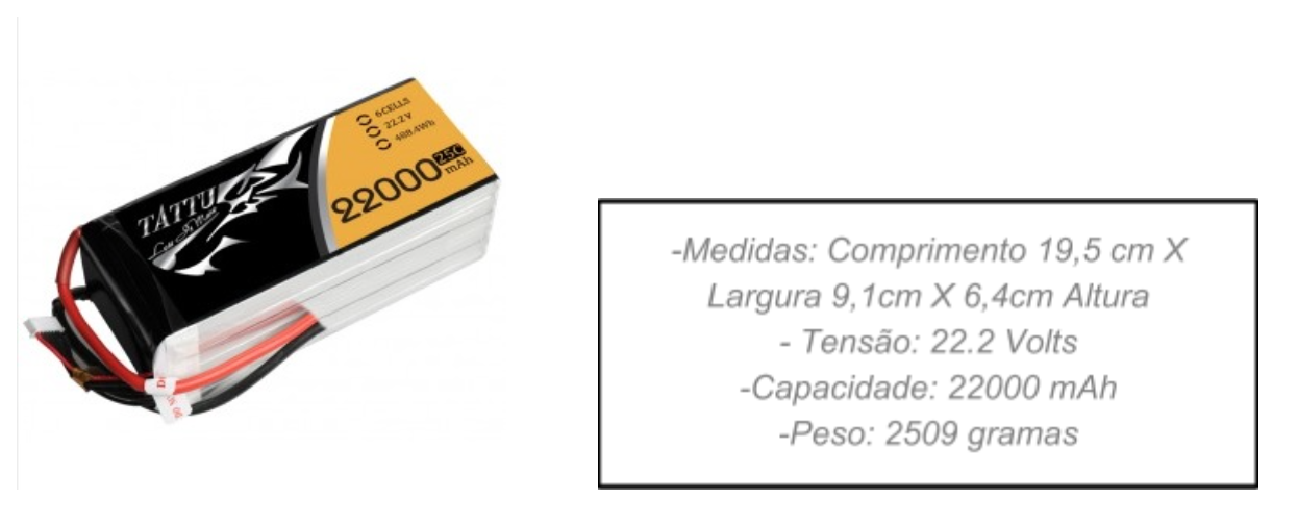
\includegraphics[keepaspectratio=true,scale=0.6]{figuras/baterialipo.eps}
    \caption{Bateria LiPO escolhida e suas especificações. Fonte: \cite{gensace}}
    \label{fig:baterialipo}
\end{figure}

\textbf{Tabela comparativa entre baterias}

\begin{figure}[H]
    \centering
	\includegraphics[keepaspectratio=true,scale=0.6]{figuras/tabelabateria.eps}
    \caption{Tabela comparativa de baterias.}
    \label{fig:tabelabateria}
\end{figure}


\subsubsection{Cálculo da autonomia e taxa de descarga do EmerVant}

Para o cálculo da autonomia de voo do EmerVant, baseamos em fórmulas sobre física e eletricidade, onde pudemos calcular a densidade da energia (wh/kg) através da tensão (V), capacidade (mA-h) e o peso da bateria(kg). 

Por seguinte, para o cálculo da autonomia, que é a duração em horas que funcionará a bateria sem recarga, considera-se que a densidade de energia da bateria que escolhemos para alimentar os motores do Drone é o que vai definir a autonomia de voo calculando a energia total armazenada na bateria,a potencia de saída, o tempo de uma hora, o empuxo especifico, empuxo total e energia total, necessária para manter o Drone voando por uma hora. Considerando que o peso total estimado do EmerVant é de 8389g, sendo:

\begin{itemize}
\item 2509g da bateria;
\item 2600g (8 bracos), onde 1 braço = 325g (Incluindo motor e hélice);
\item 1200g do desfibrilador;
\item 750 g do respirador;
\item 1330 do Peso Frame central (esqueleto);
\item 38g da placa controladora PIXHAWK.
\end{itemize}

Também foi calculada a taxa de descarga (mA) que encontra-se por regra, estandardizada relativamente à capacidade total de armazenamento da bateria e a um dado período de tempo. Sua vida útil, que é o período em que a bateria funciona em modo eficiente, será em média de 500-1000 vezes.

Considerando a tensão elétrica (V) de  22.2 V e a capacidade (amp-hora ou mA-h) de 22.000mA-h, temos que: 

\begin{equation}
Quantidade de energia = V*C => 22.2V * 22Ah = 488.4Wh
\end{equation}

Substituindo na fórmula da densidade de energia: 

\begin{equation}
Densidade de energia = \frac{quantidade de energia}{P(bateria)} => \frac{488,4wh}{2,509kg} = 194,65 Wh/g.
\end{equation}

O cálculo da autonomia foi baseado na fórmula $ET=\frac{TT}{TEt}$, onde é composta por:

\begin{itemize}
\item E (Energia total armazenada na bateria) - É a corrente que a bateria pode oferecer durante T = 1h.
\item P (Potência de saída) - É a corrente (Amperes) multiplicada pela tensão (Volts). Em fórmula P=I*V.
\item T (Tempo) - Para definição de parâmetros, é considerado 1 hora.
\item TE (Empuxo Específico) - Este parâmetro indica quantos gramas de empuxo são obtidos para cada Watt de potência entregue ao motor. Seleciona-se a pior condição para o motor do tipo(dada por tabela) que será de 7.69 g/W.
\item TT (Empuxo total) - Usa-se a média entre a potência para subida e descida, ou seja, considera-se o valor médio de potência para o Drone parado no ar. Sendo assim seu TT seria igual ao valor do Peso(8427N).  
\item ET (Energia total) - Energia necessária para manter o Drone voando por uma hora. 
\end{itemize}

Aplicando na fórmula, tem-se:

\begin{equation}
ET=\frac{TT}{TE*1h} => \frac{8427}{7.69*1h} = 1095,8 Wh.
\end{equation}

Portanto, a autonomia do Vant será determinada pela quantidade de energia contida na bateria dividida pela ET:

\begin{equation}
Autonomia = \frac{488,4Wh}{1095,8Wh *(minutos)} = 44 MINUTOS.
\end{equation}

Visto que o Vant terá consumo no motor, Esc, Sensores e controladores, a autonomia cairá, e por motivo de segurança, foi trocada a bateria de 16000 mAh para uma de com maior  tensão (Lipo 6s 22000 mAh), tentando manter a autonomia necessária para o trabalho do EmerVant (20 minutos). 

No caso da taxa de descarga (mA), onde usamos a fórmula C= I*T, onde:

\begin{itemize}
	\item C= taxa de descarga
	\item I= corrente
	\item T= período analizado
\end{itemize}

Aplicando na fórmula, obtém-se: 

\begin{equation}
C= 5,2A* 60 minutos = 312mA.
\end{equation}

\subsubsubsection{Recarga da bateria}

A carga de uma bateria é explicada de forma simples por um fenômeno químico-físico que está envolvido com a eletrólise. \cite{gibbs}

Entretanto, essa simplicidade não deve ser subestimada, pois existem detalhes nesse tipo de bateria (Lipo 6s) que precisam ser levados em consideração dependendo da sua forma de uso.

Para o recarregamento da bateria que alimentará o VANT, será utilizada uma plataforma de recarga que funcionará diretamente ligada à  central de energia da estação de controle e fornecerá a energia necessária para o recarregamento da bateria quando o VANT necessitar.

A plataforma funcionará a partir de cabos específicos que estarão ligados a central energética da estação de controle. Assim, toda vez que o VANT retornar para a central alguma pessoa capacitada conectará o mesmo à plataforma de recarga. Ao aviso de recarga da bateria do VANT, a pessoa encarregada pela central desconectará os cabos.

A bateria de polímero de Lítio caso esteja acima da temperatura normal na hora da recarga, deve ser levada para um local afastado e ventilado, para que sua temperatura normalize.A maioria dos acidentes com baterias ocorrem durante a recarga. A bateria de lítio polimerizado em comparação com as outras tem um baixo risco de acidente nesse requisito. \cite{gibbs}

As baterias de Lítio Polimerizado tem dois requerimentos em relação as suas células, primeiramente a carga deve ser limitada a um valor seguro e em segundo lugar, a voltagem da célula não deve nunca ultrapassar 4.20 Vpc (Volts por célula). \cite{gibbs}

O carregador Li-PO é um dispositivo limitador de tensão que é semelhante ao sistema de chumbo-ácido. A diferença está em uma tensão mais elevada por célula, tolerância de tensão mais apertado e a ausência de carga de flutuação em plena carga.

As baterias de polímero de Lítio não podem ser carregadas por qualquer tipo de carregador, portanto, o escolhido para atuar no sistema de recarga do EmerVant foi o carregador iMax B6 (figura \ref{fig:carregador1}), se adequa de uma forma que carrega e balanceia adequadamente vários tipos de bateria de lítio, tais como a utilizada neste projeto (LiPo 6s), Li-íon e a série de bateria LiFe.


 \begin{figure}[H]
    \centering
	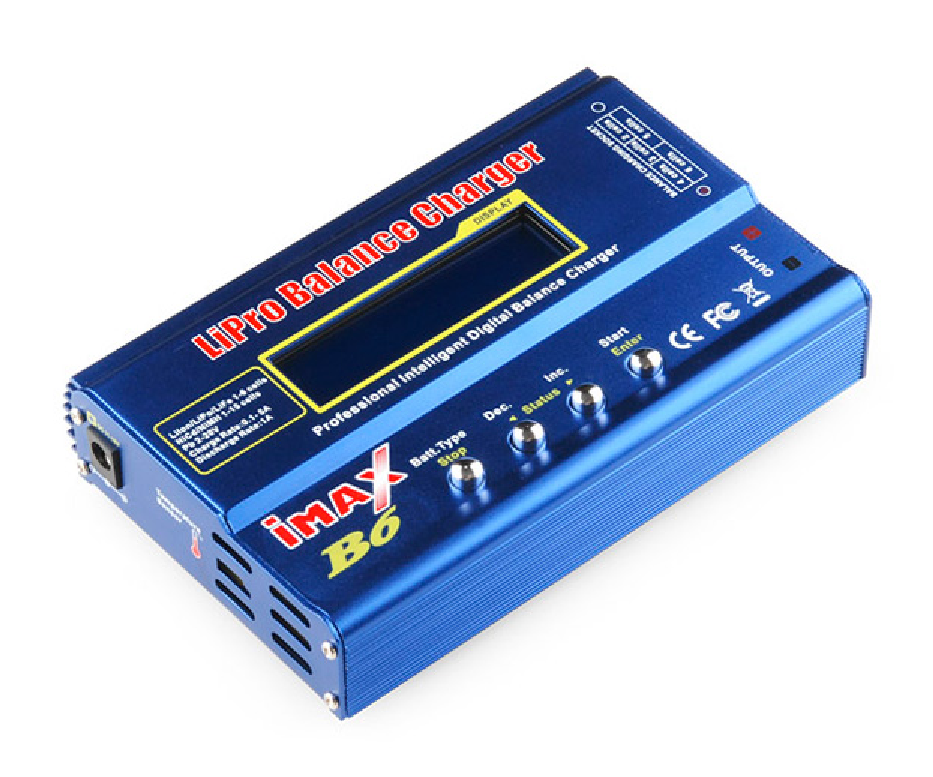
\includegraphics[keepaspectratio=true,scale=0.4]{figuras/carregador1.eps}
    \caption{Carregador iMax B6. Fonte: \cite{carregador1}}
    \label{fig:carregador1}
\end{figure}


Segundo o manual do usuário iMax B6 \cite{ibmax}, independente de qual seja a bateria de lítio usada, não será necessário se conectar a um balanceador externo para efetuar a carga de balanceamento, pois o mesmo emprega um balanceador de tensão de célula individual. Além disso, o B6 monitora e balanceia individualmente cada célula da bateria, onde apresenta uma mensagem de erro e é automaticamente interrompido caso apresente uma tensão anormal de qualquer célula individual. 

A figura a seguir mostra o menu do B6, que possui uma interface fácil de se interpretar, onde indica o carregamento e os ciclos em um processo simples, podendo ser feito de maneira rápida e precisa. O carregador não vem com a fonte de alimentação, porém contém um conector de entrada de CC que possui um \textit{plug} com garras tipo jacaré.

 \begin{figure}[H]
    \centering
	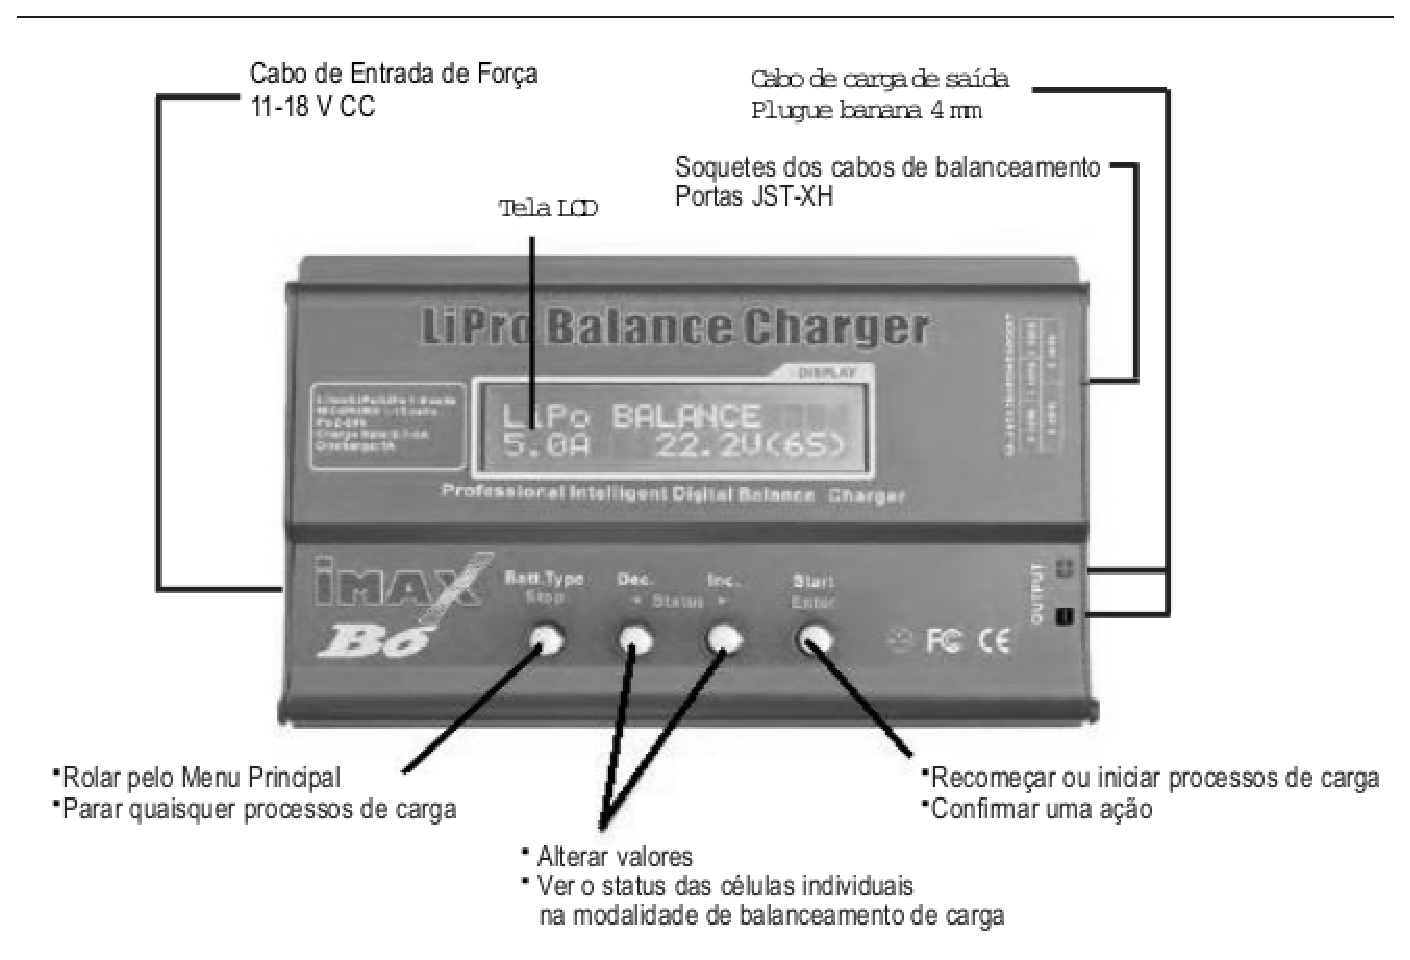
\includegraphics[keepaspectratio=true,scale=0.5]{figuras/manual.eps}
    \caption{Menu do iMax B6. Fonte: \cite{ibmax}}
\end{figure}

\section{Custos e viabilidade do projeto}
  
O EmerVant é um projeto modelo que está designado a atuar na esplanada dos ministérios em Brasília. E por esse motivo haverá produção de apenas um exemplar. O custo da produção em escala é menor que de apenas um exemplar. 

A análise dos custos foi dividida em:
\begin{itemize}
 \item Estrutura do VANT; 
 \item Comunicação;
 \item Controle;
  \item Fonte de energia;
\end{itemize}


\subsection{Custos}
Os custos de cada área e demais custos alocados no projeto, pode ser visto na Tabela \ref{custos}.
\vfill
\begin{table*}[!h]
\centering
    \caption{Custo do projeto}

\begin{tabular}{|p{0.30\linewidth}|p{0.25\linewidth}|}
\hline

Descrição & Valor (em R\$) \\ \hline

Estrutura do VANT & 14.821,13\\ \hline
Fonte energética & 2.189,64 \\ \hline
Controle do VANT & 611,97 \\ \hline
Comunicação do VANT & 63.960,00 \\ \hline
Equipamentos (Desfibrilador e reanimador) & 5.014,00 \\ \hline
Recurso humano alocado por 3 meses & 418.696,5\\ \hline
Custos mensais Central de Controle & 6.667,14\\ \hline
\textbf{Total} & 505.293,24\footnotemark + Custos mensais (6.667,14)\\ \hline

\end{tabular}
    \label{custos}
\end{table*}
\pagebreak

\footnotetext{Valores sujeitos a mudança de acordo com a cotação do dólar.}
\subsection{Análise de viabilidade econômico-financeira do projeto}

  Embora o valor tenha sido elevado, o EmerVant foi considerado um projeto viável financeiramente, visto que
  em comparação com os valores para manutenção de um helicóptero (Tabela \ref{tab:custos}) é uma alternativa
  mais em conta.



